\documentclass[10pt,twocolumn,a4paper]{article}
\usepackage[margin=17mm,columnsep=7mm]{geometry}
\usepackage[T1]{fontenc}
\usepackage[utf8]{inputenc}
\usepackage{newtxtext,newtxmath}
\usepackage{microtype}
\usepackage{graphicx}
\usepackage{booktabs}
\usepackage{array}
\usepackage{amsmath}
\usepackage{bm}
\usepackage{xcolor}
\usepackage{enumitem}
\usepackage{caption}
\usepackage{tikz}
\usepackage{url}
\usepackage{placeins}
\usepackage{dblfloatfix}
\usepackage[colorlinks=true,linkcolor=blue!50!black,citecolor=blue!50!black,urlcolor=blue!50!black]{hyperref}
\usetikzlibrary{arrows.meta,positioning,fit,backgrounds}

\captionsetup{font=small,labelfont=bf,skip=4pt}
\setlist{nosep,leftmargin=1.4em}
\setlength{\parskip}{0pt}
\setlength{\parindent}{1.2em}
\renewcommand{\arraystretch}{1.08}
\newcommand{\code}[1]{\texttt{\small #1}}
\newcommand{\pp}{\,pp}
\newcommand{\sref}[1]{\S\ref{#1}}
\newcommand{\reprolink}{\hyperref[sec:repro]{Repro.}}
\definecolor{Navy}{HTML}{17324D}
\definecolor{LightBlue}{HTML}{EAF3FB}
\definecolor{LightGold}{HTML}{FFF5DE}

\hypersetup{pdftitle={Tensor, Spectral and Raw-Waveform Learning for EEG Classification of AD and FTD},
 pdfauthor={Neeruganti Jeevan Sai; Kothapalli Tharun Chowdary; Vatipalli Abhiram; Palyam Maruthi; Shaik Moiz}}

\title{\vspace{-4mm}\textbf{Spectral, Tensor and Raw-Waveform Learning for Resting-State EEG Classification of Alzheimer's Disease and Frontotemporal Dementia Across OpenNeuro and BrainLat Cohorts}}

\author{%
\begin{tabular}{c c c}
\textbf{Neeruganti Jeevan Sai} & \textbf{Kothapalli Tharun Chowdary} & \textbf{Vatipalli Abhiram}\\
24BDS046 & 24BDS032 & 24BDS087\\[3pt]
\multicolumn{3}{c}{\begin{tabular}{c c}
\textbf{Palyam Maruthi} \hspace{2.5em} & \hspace{2.5em}\textbf{Shaik Moiz}\\
24BCS098 & 24BCS133\end{tabular}}
\end{tabular}\\[6pt]
Indian Institute of Information Technology Dharwad\\
Course: Tensor Methods for Multimodal Data Analysis and AI\\
Course instructor: Dr.\ Sibasankar Padhy}
\date{18 November 2026}

\begin{document}
\twocolumn[%
\begin{@twocolumnfalse}
\maketitle
\vspace{-6mm}
\begin{abstract}
\noindent
We study participant-level classification of Alzheimer's disease (AD), frontotemporal dementia (FTD) and cognitively normal controls (HC) from eyes-closed resting EEG. We begin with the 88 participants of OpenNeuro \code{ds004504} and benchmark tensor decompositions (PCA/NMF, CP, Tucker, Tensor Train) with SVM, random-forest and XGBoost classifiers; the best tuned model reaches $59.7\%$ balanced accuracy, while the fully automatic nested selection reaches $54.5\%$. We then add the BrainLat Argentina and Chile EEG recordings (128 channels) by spherical-spline interpolation to the common 19-electrode 10--20 montage, giving 174 participants (71 AD, 42 FTD, 61 HC). On this merged cohort, a site-normalised log-mel spectrogram SVM reaches $66.7\%$ accuracy on a fixed 27-person test split, but only about $0.49$--$0.52$ macro F1 under repeated nested participant-level cross-validation; a binary HC-versus-dementia version reaches macro F1 $0.699$ (balanced accuracy $0.703$, AUC $0.772$). CP decomposition (including graph-regularised non-negative CP), Tensor-Train and Tucker pipelines did not beat the undecomposed spectral baseline, but an interpretability analysis of their factors recovers the classical EEG signature of AD (more occipital-temporal theta, less posterior alpha) and shows that the factors mostly re-express relative band power. Finally, replacing the log-mel front end by a compact one-dimensional CNN applied directly to the raw waveform gives strikingly good validation and test numbers (test accuracy up to $70.4\%$, macro F1 $0.696$; five-fold out-of-fold macro F1 $0.643$). A per-site analysis, however, shows that this performance is concentrated in the BrainLat sites, where the CNN recognises $32/32$ controls. On OpenNeuro alone, a native-resolution CNN reaches $42.9\%$ accuracy and blending it with EEGPT reaches only $50.0\%$, so the raw-waveform result is promising but unconfirmed. All numbers come from saved experiment artefacts; no external validation was available.
\end{abstract}
\vspace{2mm}
\end{@twocolumnfalse}]

%% =====================================================================
\section{Introduction and Objectives}
\label{sec:intro}
Resting-state scalp EEG is inexpensive and non-invasive, and several studies report that Alzheimer's disease (AD) slows the dominant rhythm (more theta, less posterior alpha). Frontotemporal dementia (FTD) is harder: it overlaps AD in the spectrum, and EEG datasets containing it are small. This project, carried out for the course \emph{Tensor Methods for Multimodal Data Analysis and AI}, asks how far standard and tensor-based machine learning can separate AD, FTD and healthy controls at the \emph{participant} level, and how honest the resulting estimates are.

Our objectives were:
\begin{enumerate}[label=\textbf{O\arabic*.}]
\item Build a leakage-safe pipeline on the public 88-participant OpenNeuro cohort and benchmark tensor decompositions (PCA/NMF, CP, Tucker, Tensor Train) against spectral baselines.
\item Enlarge the cohort with the BrainLat EEG recordings, which requires harmonising a 128-electrode montage to the 19-electrode 10--20 montage.
\item Evaluate log-mel spectrogram features with SVMs for the binary (HC vs.\ dementia) and three-class (AD/FTD/HC) tasks on all 174 participants.
\item Study tensor decomposition as a dedicated component: how tensors are built, decomposed and turned into a participant-level dataset.
\item Test whether a one-dimensional CNN on the raw waveform can replace the hand-designed spectral front end.
\item Audit every result for leakage, site shift and over-optimistic selection.
\end{enumerate}

\noindent\textbf{Contributions.} (i) A documented, reproducible chain of experiments from 88 to 174 participants with participant-disjoint splits throughout; (ii) a harmonisation of OpenNeuro and BrainLat EEG and an audit of what it does and does not remove; (iii) a negative-result study of CP, Tensor-Train and Tucker methods together with an interpretability analysis of their factors; (iv) a raw-waveform CNN study whose headline numbers we then audit site by site.

\noindent\textbf{Initial tensor hypothesis.} During the initial literature review and project proposal, we identified graph-regularised non-negative tensor factorisation (G-NTF) as the main interpretable tensor experiment. The hypothesis was that non-negative factors would produce additive, readable EEG patterns, while a graph penalty based on the electrode montage would preserve spatial neighbourhoods and improve generalisation over flattening or unconstrained decomposition. This was an \emph{a priori methodological expectation}, not an experimental result. After implementation, the expectation was not supported: in repeated nested CV, G-NTF reached balanced accuracy $47.2\%$ and macro F1 $41.1\%$, below the undecomposed reference ($48.7\%$ and $45.1\%$) and no better than the shuffled-graph control ($48.5\%$ BA). Its contribution therefore became interpretability and a controlled negative result rather than improved classification.

\noindent\textbf{Benchmark position.} We do not claim a new community benchmark or state of the art. Much of the published literature studies easier binary tasks, reports window-level performance, or leaves participant aggregation and split construction unclear. Our main contribution is therefore a \emph{transparent three-class participant-level experimental baseline}: every score is tied to a stated cohort, split and selection protocol, and fixed-split results are separated from cross-validated estimates.

Figure~\ref{fig:pipeline} summarises the final processing chain.

\begin{figure*}[t]
\centering
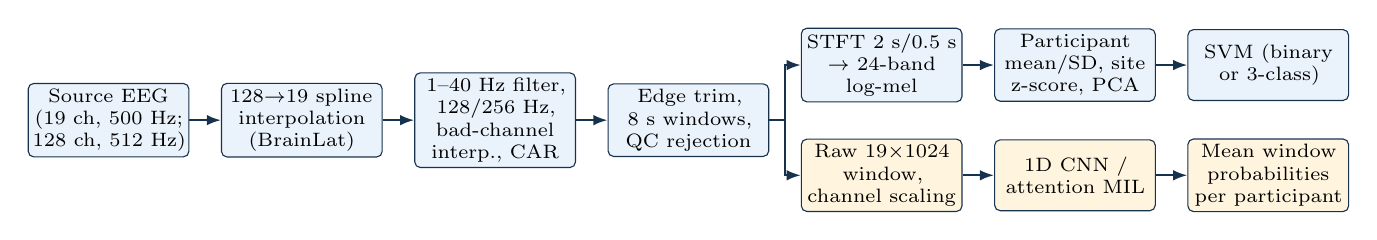
\begin{tikzpicture}[font=\scriptsize,node distance=5mm and 4mm,
 box/.style={draw=Navy,fill=LightBlue,rounded corners=2pt,align=center,minimum height=9mm,inner sep=2pt,text width=19mm},
 alt/.style={draw=Navy,fill=LightGold,rounded corners=2pt,align=center,minimum height=9mm,inner sep=2pt,text width=19mm},
 arr/.style={-{Latex[length=1.8mm]},thick,Navy}]
\node[box](a){Source EEG\\(19 ch, 500 Hz; 128 ch, 512 Hz)};
\node[box,right=of a](b){128$\to$19 spline interpolation (BrainLat)};
\node[box,right=of b](c){1--40 Hz filter, 128/256 Hz, bad-channel interp., CAR};
\node[box,right=of c](d){Edge trim, 8~s windows, QC rejection};
\node[box,right=of d,yshift=7mm](e){STFT 2~s/0.5~s $\to$ 24-band log-mel};
\node[box,right=of e](f){Participant mean/SD, site z-score, PCA};
\node[box,right=of f](g){SVM (binary or 3-class)};
\node[alt,right=of d,yshift=-7mm](h){Raw $19{\times}1024$ window, channel scaling};
\node[alt,right=of h](i){1D CNN / attention MIL};
\node[alt,right=of i](j){Mean window probabilities per participant};
\draw[arr](a)--(b);\draw[arr](b)--(c);\draw[arr](c)--(d);
\draw[arr](d.east)--++(2mm,0)|-(e.west);\draw[arr](d.east)--++(2mm,0)|-(h.west);
\draw[arr](e)--(f);\draw[arr](f)--(g);\draw[arr](h)--(i);\draw[arr](i)--(j);
\end{tikzpicture}
\caption{Final processing chain. Blue: spectral/SVM branch (Secs.~\ref{sec:logmel}--\ref{sec:threeclass}); yellow: raw-waveform branch (Sec.~\ref{sec:cnn}). Tensor decompositions (Sec.~\ref{sec:tensor}) operate on the spectral branch or on delay-embedded waveforms.}
\label{fig:pipeline}
\end{figure*}

%% =====================================================================
\section{Literature Review}
\label{sec:litreview}
\paragraph{EEG markers of AD and FTD.} Quantitative EEG studies consistently describe AD as a slowing of the resting rhythm: delta and theta power increase, posterior alpha and beta power decrease, and coherence between regions falls \cite{jeong2004,dauwels2010}. FTD is usually reported to have a comparatively preserved spectrum with smaller, more frontal changes, which makes AD and FTD harder to separate from each other than either is from controls \cite{nishida2011}. These findings motivate the spectral features used throughout this report and are the reference point for the interpretability analysis in Sec.~\ref{sec:tensorinterp}.

\paragraph{Datasets and machine-learning results.} Miltiadous \emph{et al.}\ released the 88-participant AHEPA recordings used here (OpenNeuro \code{ds004504}) \cite{miltiadous2023}, and the same group compared validation schemes on these data, showing that the choice of scheme changes the reported AD/FTD accuracy \cite{miltiadous2021}. Splits that place windows of one person in both training and test sets are a known source of optimism, which is why every split in this report is by participant. On this cohort, DICE-Net feeds band-power and coherence features to a convolution--transformer network for two binary tasks \cite{dice2023}; Rostamikia \emph{et al.}\ build a hierarchical SVM from handcrafted spectral, nonlinear and connectivity features \cite{rostamikia2024}; and Jiang \emph{et al.}\ use a two-stage EEG-microstate fusion network for dementia screening and AD/FTD differentiation \cite{jiang2026}. Outside AHEPA, Li \emph{et al.}\ factorised spectra of more than 12,000 clinical EEGs with a non-negative tensor model and related the factors to neurodegenerative disease \cite{li2024}. BrainLat \cite{prado2023} adds AD, behavioural-variant FTD and control EEG from Latin American sites, recorded with a 128-channel BioSemi system. Table~\ref{tab:lit} lists the headline results. Most are binary, and none is a merged multi-site three-class result, so we re-implemented four of them under our own protocol (Sec.~\ref{sec:litadapt}).

\begin{table}[t]
\centering\scriptsize
\caption{Published EEG studies most relevant to this project. Values are as reported by the authors and are \emph{not} directly comparable with ours (different tasks, metrics and splits).}
\label{tab:lit}
\begin{tabular}{@{}p{0.17\columnwidth}p{0.15\columnwidth}p{0.31\columnwidth}p{0.2\columnwidth}@{}}
\toprule
Study & Data & Task (validation) & Reported\\
\midrule
DICE-Net \cite{dice2023} & AHEPA, 88 & AD vs.\ CN; FTD vs.\ CN (two binary LOSO models) & 83.3\% / 75.0\% acc.\\
Rostamikia \cite{rostamikia2024} & AHEPA, 88 & Dementia vs.\ HC; AD vs.\ FTD (separate 10-fold CV) & 93.5\% / 87.8\% acc.\\
Jiang \cite{jiang2026} & AHEPA, 88 & AD/FTD/CN, three-class (LOSO) & 63.9\% BA\\
Li \cite{li2024} & 12,176 clinical EEGs & Several disease-vs.-control contrasts & AUC 0.59--0.91\\
\midrule
This work & 174, three sites & AD/FTD/HC and HC vs.\ dementia (repeated nested CV) & macro F1 $\approx$0.49 / 0.70\\
\bottomrule
\end{tabular}
\end{table}

\paragraph{Tensor methods for EEG.} Multichannel EEG is naturally a multi-way array, and CP, Tucker and related decompositions have been used to extract joint spatial, spectral and temporal signatures \cite{kolda2009,cong2015,cichocki2015}. HOSVD gives orthogonal Tucker factors \cite{delathauwer2000}, and Tensor Train offers a stable, SVD-based decomposition with controllable ranks \cite{oseledets2011}. Graph regularisation, introduced for non-negative matrix factorisation to preserve neighbourhood structure \cite{cai2011}, led to our graph-regularised non-negative CP with the electrode montage as the graph, and Li \emph{et al.}\ \cite{li2024} directly inspired the CP6 experiment.

\paragraph{Other EEG representations and deep learning.} Riemannian classifiers on channel covariance matrices \cite{barachant2012} and microstate analysis \cite{michel2018} are established EEG feature families that we use as baselines. Convolutional networks that learn temporal and spatial filters directly from the waveform can match handcrafted spectral pipelines \cite{schirrmeister2017,lawhern2018}, but a systematic review notes small cohorts, inconsistent validation and limited reproducibility in this literature \cite{roy2019}. Pretrained EEG foundation models such as EEGPT \cite{wang2024} aim to reduce the data requirement, and attention-based multiple-instance learning \cite{ilse2018} gives a principled way to pool window predictions into one participant decision.

\paragraph{Validation and site effects.} With small samples, cross-validation estimates have wide error bars \cite{varoquaux2018}, and choosing a model on the same data used to report it biases the estimate upward unless selection is nested \cite{cawley2010}. Multi-site data add batch effects, for which ComBat \cite{johnson2007} and CORAL \cite{sun2016} are standard corrections; site-wise $z$-scoring and CORAL are tested in Sec.~\ref{sec:compat}. These two concerns shape every protocol in this report.

%% =====================================================================
\section{Source Dataset and Study-I Preprocessing}
\label{sec:source}
\subsection{OpenNeuro ds004504}
\label{sec:opn}
The primary source is OpenNeuro \code{ds004504} (v1.0.9; Miltiadous et al.~\cite{miltiadous2023}): eyes-closed resting EEG from 88 participants, namely \textbf{36 AD, 23 FTD and 29 cognitively normal (CN)}, recorded at AHEPA hospital with 19 scalp electrodes (10--20), 500 Hz, A1--A2 reference. We used the authors' artefact-cleaned EEGLAB derivatives (approximately 0.5--45 Hz filtering, ASR, ICA with ICLabel component rejection \cite{pion2019}); we did not repeat these steps. Recording length ranges from about 307 s to 1,291 s, and the three groups total 29,403 s (AD), 16,753 s (FTD) and 24,434 s (CN) of data.

\subsection{Preprocessing for the 88-participant study}
\label{sec:study1prep}
Preprocessing was non-destructive: no source file was modified.
\begin{enumerate}[label=(\arabic*)]
\item \textbf{Windowing.} Recordings were cut into complete non-overlapping 4~s windows and decimated from 500 to 250 Hz ($19{\times}1000$ arrays), compatible with the 45 Hz low-pass; channel-wise window means were removed.
\item \textbf{Balanced primary cohort.} FTD, the scarcest class, set the reference: all 23 FTD participants were kept and 23 AD and 23 CN participants were matched on recording duration (and broadly on age/sex coverage), giving a 69-participant cohort.
\item \textbf{Quality control.} After common-average re-referencing, windows were excluded by fixed, label-blind rules (amplitude $\ge$400~\textmu V, adjacent-sample step $\ge$150~\textmu V, or any channel SD $<$1~\textmu V). This removed 65 windows; the clean controlled cohort contains 12,270 windows (4,090 per diagnosis).
\item \textbf{Corrections found during audit.} The first tensoriser attached a wrong electrode-label order to the data; the verified source order is Fp1, Fp2, F3, F4, C3, C4, P3, P4, O1, O2, F7, F8, T3, T4, T5, T6, Fz, Cz, Pz. EEGLAB \code{boundary} events were also found, so a 0.5~s guard was added (328 windows removed; 11,942 remain). Graph-based electrode interpretations from the first run were therefore discarded.
\item \textbf{Full-cohort extension.} Leftover windows were re-QC'd with identical rules to give an 88-participant index of 16,824 windows (AD 7,030; FTD 4,000; CN 5,794).
\end{enumerate}
\paragraph{Safeguards.} All splits are by participant; decompositions, scalers, selection and class weights are fitted on training participants only; features are pooled within a participant; no SMOTE or demographic/clinical variables are used.

%% =====================================================================
\section{Study I: The 88-Participant OpenNeuro Benchmark}
\label{sec:study1}
The first phase compared tensor and spectral representations under participant-level nested cross-validation (CV). Balanced accuracy (BA, the mean of AD, FTD and CN recall) is the main metric; chance is $33.3\%$.

\paragraph{V1: exploratory spectral tensor.} A $69{\times}19{\times}59{\times}10$ tensor (participant $\times$ channel $\times$ 1--30 Hz $\times$ recording-time decile; Welch relative power, square-root transformed) was reduced by PCA, NMF, non-negative CP, graph-regularised CP and non-negative Tucker at ranks 3/5/8 and classified with logistic regression, RBF SVM or gradient boosting (3$\times$5 CV). The best exploratory result was PCA(8)+logistic and NMF(8)+logistic at \textbf{54.1\%} BA, with FTD recall near $30\%$.

\paragraph{V2: nested TT/Tucker.} On the corrected channel order and boundary-safe index, each window became a signed log$_{10}$ PSD tensor ($19{\times}59{\times}3$). Subject-TT, window-TT, graph-smoothed TT, window-Tucker/HOSVD and spectral controls were compared with ranks 8/16/32 (Tucker $(6,8,3)$) under 3$\times$5 outer/3-fold inner nested CV. Automatic selection gave 47.3\% BA; the best family observed (Tucker) gave 56.0\%.

\paragraph{V3: raw-waveform tensors on 88 people.} Waveforms (resampled to 125 Hz) were delay-embedded into $19{\times}16{\times}485$ channel$\times$lag$\times$position tensors; TT/Tucker filters produced squared-response energies pooled per person. Automatic selection reached 52.0\% BA, the same-cohort spectral control 55.8\%, waveform Tucker 51.8\%, waveform TT 50.9\%, supervised TT 49.9\%.

\paragraph{V4: bounded classifier tuning.} Using V3's inputs and outer splits, 139 pre-frozen configurations (logistic, RBF SVM, shallow XGBoost, random forest, regularised supervised TT) were evaluated (Table~\ref{tab:study1}). The \textbf{tuned RBF SVM reached 59.7\% $\pm$ 0.9~pp BA} (this is the ``$\approx$60\%'' first result); the fully automatic selection reached 54.5\% $\pm$ 3.2~pp.

\begin{table}[t]
\centering\small
\caption{Study I (OpenNeuro only), mean balanced accuracy under participant-level CV. ``Obs.'' means best observed over candidates (optimistic); ``Auto'' means whole-pipeline nested selection.}
\label{tab:study1}
\begin{tabular}{@{}llr@{}}
\toprule
Exp.\ & Method (cohort) & BA (\%)\\
\midrule
V1 & PCA(8)+logistic, obs.\ (69) & 54.1\\
V2 & Tucker/HOSVD, obs.\ (69) & 56.0\\
V2 & Full nested auto (69) & 47.3\\
V3 & Spectral control, obs.\ (88) & 55.8\\
V3 & Full nested auto (88) & 52.0\\
V4 & Tuned RBF SVM, obs.\ (88) & \textbf{59.7}\\
V4 & Tuned random forest (88) & 58.3\\
V4 & Tuned XGBoost (88) & 57.6\\
V4 & Tuned logistic (88) & 54.6\\
V4 & Full nested auto (88) & 54.5\\
\bottomrule
\end{tabular}
\end{table}

\paragraph{Binary variant (V6).} Collapsing AD and FTD into ``dementia'' (59 vs.\ 29) with 36 fixed pipelines selected by macro F1 gave, over three repeats of 5-fold CV, \textbf{75.0\%} accuracy, macro F1 $0.718$, dementia recall $80.8\%$ and control specificity $63.2\%$. The trivial always-dementia rule has $67.0\%$ accuracy but macro F1 $0.401$, which is why macro F1 is the primary binary metric.

\paragraph{Take-away.} Even the best OpenNeuro-only model stays near 60\% BA, FTD recall is only $\approx$30--43\%, and the 23 FTD participants cannot be enlarged by adding windows. This motivated adding a second cohort.

%% =====================================================================
\section{Adding BrainLat: Harmonisation and Preprocessing}
\label{sec:brainlat}
\subsection{BrainLat EEG}
\label{sec:brainlatdata}
BrainLat \cite{prado2023} contains 128-channel BioSemi, 512 Hz, eyes-closed resting EEG from sites in Argentina (AR) and Chile (CL), each about 10 minutes. We used the AD, behavioural-variant FTD and healthy-control folders. Of the relevant headers, 14 HC recordings lack their external \code{.fdt} signal files and were unusable, leaving \textbf{86 BrainLat participants (AR 48, CL 38)}. The merged cohort is in Table~\ref{tab:cohort}.

\begin{table}[t]
\centering\small
\caption{Merged cohort (174 participants).}
\label{tab:cohort}
\begin{tabular}{@{}lcccc@{}}
\toprule
Site & AD & FTD & HC & Total\\
\midrule
AHEPA (OpenNeuro) & 36 & 23 & 29 & 88\\
AR (BrainLat) & 16 & 13 & 19 & 48\\
CL (BrainLat) & 19 & 6 & 13 & 38\\
\midrule
Total & 71 & 42 & 61 & 174\\
\bottomrule
\end{tabular}
\end{table}

\subsection{Electrode interpolation}
\label{sec:interp}
OpenNeuro provides 19 measured electrodes; BrainLat provides 128. To use one model, BrainLat is projected to the 19-electrode 10--20 montage. We load each recording in MNE-Python \cite{gramfort2013}, attach the standard \code{biosemi128} montage (verifying that all 128 channel names match), and call \code{interpolate\_to} with the 19-channel 10--20 target montage using \textbf{spherical-spline} interpolation \cite{perrin1989}. In spherical splines, the potential at a target location $\mathbf r$ is
\begin{equation}
V(\mathbf r)=c_0+\sum_{i=1}^{128}c_i\,g\!\left(\cos\angle(\mathbf r,\mathbf r_i)\right),
\end{equation}
where $g$ is a Legendre-series kernel on the unit sphere and the coefficients $c_i$ are obtained from the measured potentials. After interpolation, standard 10--20 head coordinates are re-attached so later recording-specific channel repair has valid geometry. Legacy OpenNeuro labels T3/T4/T5/T6 are renamed to T7/T8/P7/P8 so both sources share one channel order.

\paragraph{Caveat.} Interpolated BrainLat channels are \emph{estimates}, not measurements. In a BrainLat-only ablation (86 people, binary, nested CV) we compared native 128 channels (macro F1 $0.614$), native-19-sensor subset ($0.566$), the legacy interpolation ($0.599$) and an origin-aligned interpolation ($0.554$). The interpolated 19-channel version did not underperform the native 19-sensor subset and was within CV noise of the full 128-channel result, but it is not a substitute for dense sampling.

\subsection{Preprocessing of the merged cohort}
\label{sec:prep}
Two streams were built from the same recordings.
\begin{enumerate}[label=(\arabic*)]
\item Map both sources to the common 19 channels (Sec.~\ref{sec:interp}); band-pass 1--40 Hz; resample to 128 Hz (256 Hz for later binary/compatibility work).
\item \textbf{Moderate stream (used for the main models).} Average (common-average) reference; remove 10 s from each recording edge; non-overlapping \textbf{8-second windows}; reject windows with a flat, extreme-amplitude, high-derivative, impulsive or non-finite channel; keep at most 40 windows per person; reject windows near EEGLAB boundary/BAD intervals (2 s guard) in the later binary experiment.
\item \textbf{Advanced stream (ablation).} Additionally detect bad channels robustly (amplitude, peak-to-peak, 30--40 Hz noise ratio, correlation with neighbours), interpolate at most four per recording with spherical splines, and remove at most two ocular ICA components when correlation, frontal loading and kurtosis jointly indicate an eye component.
\end{enumerate}
The advanced stream interpolated 238 channels in 114 of 174 recordings and removed 87 ICA components from 76 recordings; it kept 6,719 windows after rejecting 277. Paired repeated-CV showed that it \emph{lowered} macro F1 by 1.98~pp (Sec.~\ref{sec:threeclass}), so the moderate stream is the working preprocessing.

\subsection{Spectral representation}
\label{sec:spectral}
Each window is transformed by a short-time Fourier transform (2~s Hann window, 0.5~s hop, 1--40 Hz), giving a $19{\times}79{\times}13$ log-power tensor. Power is compressed by a bank of $M=24$ mel-spaced triangular filters (mel scale $m=2595\log_{10}(1+f/700)$) to a $19{\times}24{\times}13$ \textbf{log-mel} tensor, and each window is centred by its median log power to suppress recording-gain differences. A participant is summarised by the mean and standard deviation over windows and frames of every electrode--band cell, producing $19{\times}24{\times}2=912$ features.

\subsection{Cross-cohort compatibility audit}
\label{sec:compat}
Compatibility was audited on all 174 people after matching reference (CAR), band (1--40 Hz) and rate (256 Hz). Even after matching, a classifier could still identify the dataset with $90.6\%$ balanced accuracy (99.8\% with the original derivatives), and the sites differ in reference (A1--A2 versus average), upstream cleaning and age (median AD age 67 in AHEPA vs.\ 76 in BrainLat). Site-wise $z$-scoring or CORAL alignment reduced dataset identifiability (probe $\approx$50\%) but also lowered HC-vs-dementia macro F1 from $82.4\%$ to $63.9$--$66.8\%$.

The audit shows that signal matching is possible but that the two derivatives are not interchangeable, which is why every later model refits site normalisation on training participants only and why we report site-wise results.

%% =====================================================================
\section{Log-Mel Spectrogram + SVM Pipeline}
\label{sec:logmel}
Our main model family classifies the 912 participant features with a support-vector machine \cite{cortes1995}. All steps are refitted inside each training fold:
\begin{enumerate}[label=(\arabic*)]
\item \textbf{Site normalisation:} each feature is standardised with the mean and SD of training participants from the \emph{same site} (AHEPA, AR, CL); validation and test people never contribute statistics.
\item \textbf{Scaling and PCA} (10--80 components or none).
\item \textbf{SVM} with linear or RBF kernel, $C\in[10^{-3},10^{2}]$, class-balanced weights (optionally an extra FTD boost) and, for binary work, a decision-score threshold chosen on inner out-of-fold predictions.
\end{enumerate}
We report participant-level metrics (all windows of a person are aggregated first). Two evaluation protocols are used throughout:
\begin{itemize}
\item \textbf{Fixed split}: 121 train / 26 validation / 27 test participants stratified by site$\times$diagnosis (test: 11 AD, 6 FTD, 10 HC). One test participant is worth $3.7$ accuracy points, and the test set was inspected repeatedly, so fixed-split numbers are exploratory.
\item \textbf{Repeated nested CV}: $5{\times}5$ or $3{\times}5$ outer participant-level folds stratified by site$\times$diagnosis, with inner folds for all selection. This is our primary evidence.
\end{itemize}

%% =====================================================================
\section{Binary Classification on All 174 Participants}
\label{sec:binary}
\textbf{Task.} HC (61) versus dementia (71 AD + 42 FTD = 113). The primary metric is macro F1 because the dementia class is the majority.

\textbf{Search.} A frozen 256-candidate seeded search covered sampling rate (128/256 Hz), window length (2/4/6/8~s), STFT window (1/2/3~s), hop (0.25/0.5/1~s), mel filters (16/24/32), summaries (mean/SD or +median/IQR), site adjustment (none, centring, $z$-score), scaler, PCA, kernel, $C$, $\gamma$, class weights and threshold. At most 320 accepted seconds per person were used at every window length. Validation used 3 repeats of 5 outer folds with 3 inner folds; every configuration choice was made inside the training folds.

\begin{table}[t]
\centering\small
\caption{Binary (HC vs.\ dementia), 174 participants, 3$\times$5 nested CV (mean over repeats; repeat SD in brackets).}
\label{tab:binary}
\begin{tabular}{@{}lr@{}}
\toprule
Metric & Value\\
\midrule
Macro F1 & 0.699 (0.003)\\
Balanced accuracy & 0.703 (0.002)\\
Accuracy & 0.720 (0.007)\\
HC recall (specificity) & 0.645 (0.025)\\
Dementia recall & 0.761 (0.023)\\
ROC AUC & 0.772 (0.022)\\
\midrule
Always-dementia baseline: macro F1 / acc. & 0.394 / 0.649\\
Macro F1 95\% CI (conditional bootstrap) & 0.647--0.752\\
Fixed 128 Hz / 256 Hz control macro F1 & 0.693 / 0.693\\
\bottomrule
\end{tabular}
\end{table}

\textbf{Results.} Table~\ref{tab:binary} and Fig.~\ref{fig:binaryresults} show macro F1 $0.699$ and balanced accuracy $0.703$, clearly above the trivial baseline but far from clinical grade; healthy controls are the harder class to recognise ($64.5\%$). By site, macro F1 was $0.760$ in AHEPA, $0.636$ in AR and $0.633$ in CL, so performance is weaker in the interpolated BrainLat data. The two sampling rates gave identical control scores (the 128 Hz signal is a down-sampled copy of the 256 Hz one, and the 1--40 Hz band is fully represented at both); the search picked 256 Hz in 7 and 128 Hz in 8 of 15 outer folds. The dementia-versus-control task was thus the easiest formulation, but it does not separate AD from FTD.

\begin{figure*}[!tbp]
\centering
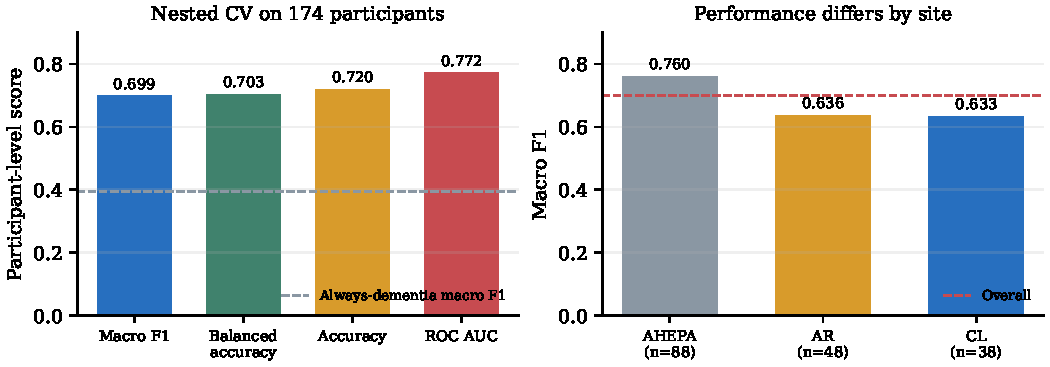
\includegraphics[width=0.92\textwidth]{figures/fig_binary_results.pdf}
\caption{Binary HC-versus-dementia evidence. Left: repeated nested-CV metrics; the dashed line is the macro F1 of the always-dementia rule. Right: site-wise macro F1 from the same participant-level predictions. The model is useful above the trivial baseline, but its performance is materially lower at the two BrainLat sites.}
\label{fig:binaryresults}
\end{figure*}
\FloatBarrier

%% =====================================================================
\section{Three-Class Classification (AD / FTD / HC)}
\label{sec:threeclass}
\subsection{Fixed-split results}
\label{sec:fixedsplit}
On the 121/26/27 split, selected models gave Table~\ref{tab:fixed}; Fig.~\ref{fig:fixedconfusions} shows the confusion matrices. The site-normalised log-mel SVM (validation-selected: moderate cleaning, all 19 electrodes, 20 PCA components, linear SVM, $C{=}0.1$) reached $66.7\%$ accuracy (18/27) and macro F1 $64.3\%$, an $11$-point gain over the earlier hierarchical SVM; site normalisation gave the largest single gain. The EEGPT transfer-learning variants are summarised separately in Sec.~\ref{sec:eegpt}. Longer CNN training raised validation macro F1 to $72.4\%$ but \emph{lowered} test macro F1 to $40.7\%$, a clear example of validation overfitting on 26 people.

\begin{table}[t]
\centering\small
\caption{Three-class, fixed 27-person test split (exploratory).}
\label{tab:fixed}
\begin{tabular}{@{}lrrr@{}}
\toprule
Model & Acc.\ & F1 & Recall A/F/H\\
\midrule
Log-STFT SVM (advanced) & 40.7 & 40.2 & 36/33/50\\
Log-mel CNN (2D) & 59.3 & 52.1 & 64/17/80\\
Log-mel CNN, long training & 51.9 & 40.7 & 64/0/70\\
Filter-bank Riemannian SVM & 48.1 & 42.3 & 27/17/90\\
\textbf{Site-norm.\ log-mel SVM} & \textbf{66.7} & \textbf{64.3} & 73/50/70\\
\bottomrule
\end{tabular}
\end{table}

\begin{figure*}[!tbp]
\centering
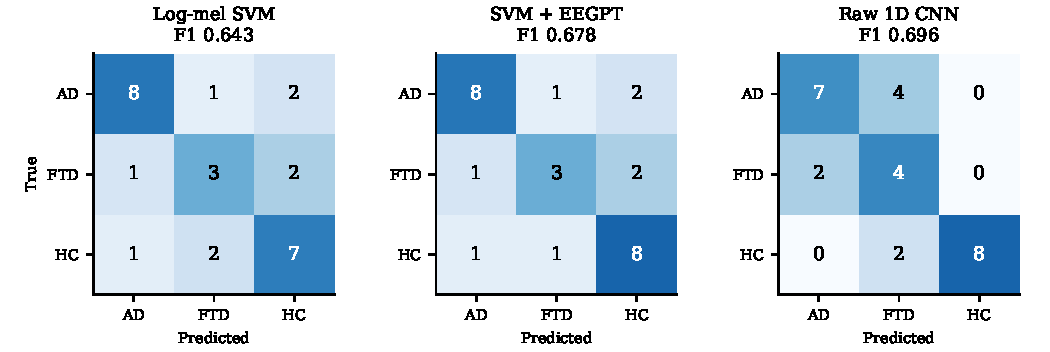
\includegraphics[width=0.86\textwidth]{figures/fig_threeclass_confusions.pdf}
\caption{Fixed-split confusion matrices for the three models most often compared in the report. Counts are participant-level. The EEGPT blend gains one HC over the log-mel SVM; the raw CNN gains FTD recall but redirects four AD participants to FTD.}
\label{fig:fixedconfusions}
\end{figure*}

\subsection{Honest estimates: repeated nested CV}
\label{sec:repeatedcv}
The same SVM, replayed over 50 repeated test folds, averaged only $48.1$--$49.0\%$ macro F1 (range $33.3$--$66.0\%$); the fixed-split $64.3\%$ sits at the optimistic edge of that distribution. Table~\ref{tab:repeated} collects the repeated-CV evidence on the 174 participants. Electrode subsets (5/8/12/19 electrodes) did not help: the eight-electrode model matched the full montage ($49.1\%$ vs.\ $49.0\%$ macro F1) but the chosen eight changed from fold to fold (the most frequent, T8 and O2, appeared in only 62\% and 60\% of folds). Grouped permutation importance ranked theta (4--8~Hz) first (6.1~pp macro-F1 drop), then beta (4.0) and gamma (3.1); alpha contributed $0.9$ and delta $0.1$. The FTD class remains the bottleneck (recall $27$--$36\%$), and a stable 29\% of FTD participants were mislabelled by at least 80\% of 23 model variants, mostly as AD. Fig.~\ref{fig:threeclassprogression} summarises macro F1 across the principal experiments, keeping fixed-split and cross-validated results apart. Published methods adapted to the same task are compared in Sec.~\ref{sec:litadapt}.

\begin{table}[t]
\centering\small
\caption{Three-class repeated participant-level CV on 174 people (macro F1, mean $\pm$ fold SD).}
\label{tab:repeated}
\begin{tabular}{@{}lr@{}}
\toprule
Model (reference) & Macro F1 (\%)\\
\midrule
Site-norm.\ SVM, 19 electrodes, 50 folds & $49.0\pm6.6$\\
Compact features, moderate cleaning & $50.9\pm7.6$\\
Compact features, advanced cleaning & $48.9\pm8.0$\\
Fixed 50/50 fusion of both streams & $51.4\pm8.9$\\
Compact-feature random forest & $51.7\pm7.8$\\
\bottomrule
\end{tabular}
\end{table}

\begin{figure*}[!tbp]
\centering
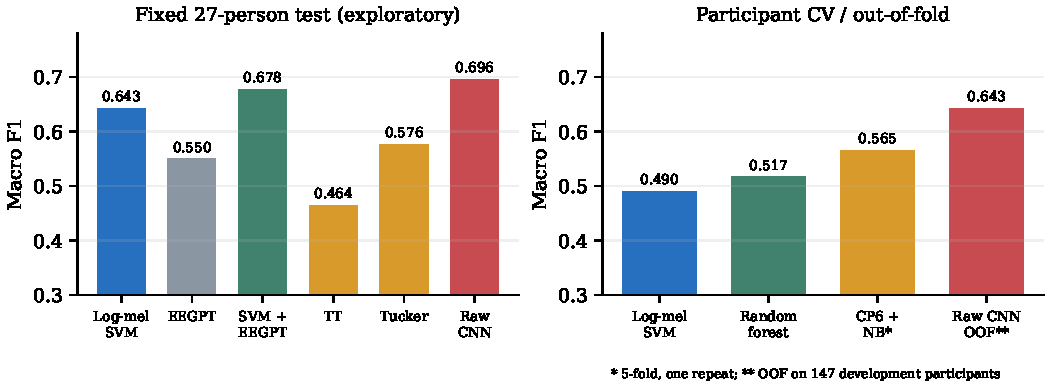
\includegraphics[width=0.92\textwidth]{figures/fig_threeclass_progression.pdf}
\caption{Three-class macro F1 across the principal experiments. Protocols are separated deliberately: the left panel uses the repeatedly inspected 27-person fixed test split, whereas the right panel uses participant-level cross-validation or out-of-fold predictions. Bars across panels must not be ranked as if they were produced by one evaluation.}
\label{fig:threeclassprogression}
\end{figure*}
\FloatBarrier

%% =====================================================================
\section{Comparison with Adapted Literature Methods}
\label{sec:litadapt}
Four published approaches were re-implemented on all 174 participants with shared outer participant folds (five folds, one prediction per person); they are adaptations, not exact reproductions: Li-style CP rank-6 + Gaussian naive Bayes \cite{li2024} ($60.3\%$ acc., $56.5\%$ BA, FTD recall $31.0\%$), a Rostamikia-style hierarchical handcrafted-feature SVM \cite{rostamikia2024} ($55.2\%$ / $52.5\%$), DICE-Net adapted to three classes \cite{dice2023} ($51.1\%$ / $48.3\%$) and a Jiang-style microstate-CNN cascade \cite{jiang2026} ($41.4\%$ / $42.7\%$). Even the best has an FTD recall of about 31\%. These results should be read as matched protocol controls, not claims that the original papers reported these three-class numbers.

\subsection{Why the literature scores did not transfer}
\label{sec:literature-gap}
The apparent gaps are partly comparisons of \emph{different endpoints}, and partly losses observed after changing the data and implementation. Our endpoint is a single held-out AD/FTD/HC decision for each of 174 people. Eighty-eight people are from AHEPA/OpenNeuro and 86 from BrainLat Argentina/Chile. Every fold mixes these sources in training and test, and all fitting and feature selection occur inside training folds. The original papers did not evaluate this exact merged-cohort task. The following distinguishes measured evidence from mechanisms that still need ablation.

\noindent\textbf{Li CP6 + naive Bayes.} Li \emph{et al.}\ fitted six non-negative spectral factors to 12,176 clinical EEG recordings and reported AUCs $0.59$--$0.91$ for several patient-versus-control contrasts, and AUC $0.61$ for AD dementia versus dementia with Lewy bodies \cite{li2024}. These are \emph{binary AUCs}, not three-class accuracy and not AD versus FTD. We refitted the factorization in each training fold (roughly 139 people) to avoid exposing the test participants during representation learning. This removes the paper's large external pool for learning stable factors; it also changes the frequency range from 1--45 to 1--40 Hz and uses a bounded L-BFGS-B solver. Three of five final CP fits had no converged start within 500 iterations and three initializations. Thus the smaller factor-learning sample and incomplete optimization are concrete possible losses, while the metric and disease contrasts prevent a numerical accuracy-gap claim. In our held-out predictions, 22/42 FTD participants were labelled AD, and accuracy among the 88 AHEPA participants was $47.7\%$, versus $60.3\%$ overall. The latter is a mixed-training-fold subgroup result, not an AHEPA-only reproduction.

\noindent\textbf{Rostamikia hierarchical SVM.} The paper's $93.5\%$ is dementia versus HC and its $87.8\%$ is AD versus FTD, each a \emph{separate binary ten-fold CV task} on 88 people \cite{rostamikia2024}. Our reported $55.2\%$ is the harder \emph{composed three-class} decision: stage 1 can reject a dementia patient as HC before stage 2 sees them. From our final confusion matrix, 25/113 dementia participants were sent to HC, while 15/61 controls were sent to a dementia label. Among the 88 dementia participants routed to a dementia label, only 50 received the correct AD/FTD subtype ($56.8\%$); this conditional figure is not directly comparable with the paper's separately evaluated AD/FTD classifier. We also used Butterworth rather than db4 wavelet bands, bounded estimators for nonlinear features, and fold-specific selection and scaling. These differences can change the frontal/connectivity features the SVM sees; we cannot isolate their individual effect from this run.

\noindent\textbf{DICE-Net.} Its reported $83.28\%$ AD-versus-control and $74.96\%$ FTD-versus-control accuracies come from \emph{two binary LOSO models}, not a single three-class model \cite{dice2023}. We replaced the head with three logits, so AD and FTD compete as well as each competing with HC. Our three-class model correctly identified only 11/42 FTD people; 14 were called AD and 17 HC. The original used ASR/ICA cleaning, approximately 30-second input windows, and its own power/coherence calculation. We used common harmonization, 31-second windows with 30 feature frames, a Morlet coherence implementation, and a corrected batch-first transformer. The AHEPA subgroup accuracy was $54.5\%$ even though the original study used the AHEPA cohort; adding BrainLat alone therefore cannot account for the full difference. The published LOSO split is participant-disjoint, so we do not attribute its higher binary scores to leakage.

\noindent\textbf{Jiang microstate cascade.} This is the closest endpoint match: the original reported $63.9\%$ three-class \emph{balanced accuracy} under participant-level LOSO on 88 AHEPA subjects, versus our $42.7\%$ on the merged cohort \cite{jiang2026}. Our AHEPA subgroup reached only $48.8\%$ balanced accuracy, while Argentina and Chile reached $35.7\%$ and $39.1\%$, respectively. Site transfer appears to add difficulty, but the AHEPA result shows it is not the only issue. The original used 10-second/256-Hz epochs, 0.5--45 Hz filtering and many overlapping epochs; ours used 8-second/128-Hz windows and 1--40 Hz filtering, capped maps/windows for template learning, and reimplemented architecture details because author code was unavailable. Shorter and sparser sequences may lose microstate transitions; the result does not establish which change dominates. Our errors are concentrated in AD: only 18/71 AD people were correct, with 30 called FTD and 23 HC, whereas FTD recall was $45.2\%$.

\noindent\textbf{What the evidence supports.} Binary-versus-three-class and AUC-versus-accuracy differences are known reasons the headline numbers cannot be subtracted from ours. Mixed-site acquisition, common preprocessing, smaller factor-learning data, bounded optimization and model reimplementation are specific, plausible sources of loss. We have not measured each cause independently. In particular, the moderate preprocessing path did not explicitly reject EEGLAB boundary annotations, which can degrade signal quality but is not evidence of participant leakage. To quantify causes, the next controlled comparison would hold the AHEPA subjects, three-class endpoint and participant split fixed while changing one of preprocessing, feature estimator or model implementation at a time, then separately test BrainLat transfer. Until then, these are paper-inspired internal controls rather than failed exact replications or evidence that the original papers' results are invalid.

%% =====================================================================
\section{EEGPT Transfer Learning (Brief)}
\label{sec:eegpt}
We also tried a pretrained EEG foundation model, EEGPT \cite{wang2024}. The official 58-channel, 4~s, 256 Hz checkpoint (checksum verified) accepts our 19 named electrodes directly. We used 6,913 accepted 4~s windows from all 174 participants (in microvolts, resampled to 256 Hz), trained a participant-level attention head on the frozen encoder, and then fine-tuned only the last two transformer blocks at a lower learning rate (best epoch 9). On the fixed split it reached $63.0\%$ accuracy (macro F1 $55.0\%$, FTD recall $17\%$); a validation-selected equal-weight blend of its probabilities with the site-normalised SVM gave $70.4\%$ accuracy and macro F1 $67.8\%$ (FTD recall $50\%$), one participant better than the SVM alone. Appending two new transformer blocks left validation F1 unchanged ($64.1\%$) but cut test macro F1 from $55.0\%$ to $46.9\%$, so deeper heads were rejected.

\begin{table}[t]
\centering\small
\caption{EEGPT: fixed split and repeated-CV re-check (frozen embeddings, $5{\times}5$ nested CV, 174 people).}
\label{tab:eegpt}
\begin{tabular}{@{}lr@{}}
\toprule
Setting & Macro F1 (\%)\\
\midrule
Fixed split: SVM + EEGPT blend & 67.8\\
Fixed split: EEGPT alone & 55.0\\
\midrule
CV: spectral SVM (reference) & $51.3\pm9.1$\\
CV: frozen EEGPT, unnormalised input & $60.1\pm7.9$\\
CV: EEGPT, recording-gain normalised & $49.7\pm7.6$\\
CV: EEGPT, window/channel $z$-score & $48.9\pm8.9$\\
\bottomrule
\end{tabular}
\end{table}

The repeated-CV re-check (Table~\ref{tab:eegpt}) is the important result. With the unnormalised input scale, frozen EEGPT embeddings looked about 9 points better than the spectral SVM, but once the inputs were normalised per recording or per window the advantage vanished (BrainLat control recall fell from $0.96$ to about $0.55$). We therefore treat the $70.4\%$ blend as unconfirmed and do not pursue EEGPT further.

%% =====================================================================
\section{Tensor Decomposition: CP and Tensor Train}
\label{sec:tensor}
\subsection{Why tensors, and the common recipe}
\label{sec:tensorrecipe}
EEG naturally forms a multi-way array (electrode $\times$ frequency $\times$ statistic or time $\times$ participant), and flattening it discards structure. A tensor $\mathcal X\in\mathbb R^{I_1\times\cdots\times I_N}$ can be compressed by low-rank models whose factors are shared across participants \cite{kolda2009}. In every tensor pipeline the same four steps build the participant-level dataset:
\begin{enumerate}[label=(\arabic*)]
\item windows $\to$ spectral array per window (log-mel or PSD);
\item pool windows inside each participant (never across participants) into one participant tensor;
\item \textbf{fit the decomposition on training participants only}, which fixes a shared basis;
\item project every participant (train, validation, test) onto that fixed basis to obtain a short feature vector, then standardise and classify.
\end{enumerate}
We used two principal families, CP decomposition (CPD) and Tensor Train (TT), plus Tucker/HOSVD variants for comparison.

\subsection{CP decomposition (CPD) and the G-NTF experiment}
\label{sec:cp}
A rank-$R$ CP model approximates $\mathcal X$ by a sum of $R$ rank-one tensors,
\begin{equation}
\mathcal X\approx\sum_{r=1}^{R}\mathbf a_r\circ\mathbf b_r\circ\mathbf c_r\circ\cdots,
\end{equation}
where each column $\mathbf a_r$ of the participant factor $\mathbf A\in\mathbb R^{N\times R}$ is the activation of component $r$ in every person, and the other factors are shared patterns (electrode, frequency, statistic). The $R$ activations of a participant are its features.

\emph{Dataset construction (CP on spectral tensors).} We used two datasets.
(i) \textbf{CP on PSD (Li-style, CP6).} A channel$\times$frequency log-PSD summary ($19\times40$, integer 1--40~Hz) per participant is min/max-normalised and stacked to $174\times19\times40$; a non-negative CP of fixed rank $R{=}6$ gives six activations per person, classified with Gaussian naive Bayes.
(ii) \textbf{Graph-regularised non-negative CP (G-NTF).} This was the experiment proposed from the initial literature review. We expected the electrode-graph constraint to favour spatially coherent factors and the non-negative participant embeddings to make both classification and interpretation more reliable. Window log-mel power is converted back to positive power, normalised by total electrode/mel power and square-rooted; per participant the mean, SD, median and IQR over windows/frames are stacked, giving $\mathcal X\in\mathbb R^{174\times19\times24\times4}$ (participant $\times$ electrode $\times$ mel band $\times$ statistic). Its model is
\begin{equation}
\hat X_{ncfs}=\sum_{r}A_{nr}B_{cr}F_{fr}S_{sr},
\end{equation}
\begin{equation}
\min\ \tfrac12\tfrac{\|\mathcal X-\hat{\mathcal X}\|^2}{\|\mathcal X\|^2}+\tfrac{\lambda}{2R}\mathrm{tr}(\mathbf B^{\!\top}\mathbf L\mathbf B),
\end{equation}
with all factors non-negative, unit-norm columns for $\mathbf B,\mathbf F,\mathbf S$ \emph{inside} the objective (removing a scale loophole that let the penalty be evaded by shrinking $\mathbf B$), exact gradients checked by finite differences, optimisation by bounded L-BFGS-B with three initialisations, and $\mathbf L$ the Laplacian of a four-neighbour scalp-distance graph. A plain NTF ($\lambda{=}0$), a graph-shuffled control and a TT control were run on identical folds.

\emph{Projecting held-out people.} Factors $\mathbf B,\mathbf F,\mathbf S$ are frozen after training. For a new participant tensor $\mathcal X_n$ we solve the non-negative least-squares problem $\min_{\mathbf a\ge0}\|\mathcal X_n-\sum_r a_r\,\mathbf b_r\circ\mathbf f_r\circ\mathbf s_r\|^2$ to obtain $\mathbf a=A_{n,:}$; site means are subtracted \emph{after} decomposition using training embeddings only, which preserves non-negativity. The embedding goes through PCA/standardisation and an SVM (ranks 3/5/8/12/16, $\lambda\in\{10^{-3},\dots,1\}$, linear/RBF, nested CV).

\subsection{Tensor Train (TT)}
\label{sec:tt}
A TT decomposition \cite{oseledets2011} writes $\mathcal X(i_1,\dots,i_N)=\mathbf G_1(i_1)\mathbf G_2(i_2)\cdots\mathbf G_N(i_N)$ with cores $\mathcal G_k\in\mathbb R^{r_{k-1}\times I_k\times r_k}$, $r_0{=}r_N{=}1$, computed by sequential truncated SVDs (TT-SVD). Unlike CP, TT ranks are bounded by unfolding ranks and the algorithm is non-iterative and stable.

\emph{Dataset construction (summary-first TT).} For each participant we stacked four statistics (mean, SD, median, IQR) of the log-mel values over all windows and frames, giving $\mathcal X_p\in\mathbb R^{19\times24\times4}$ and a cohort tensor $174\times19\times24\times4$. After training-only site normalisation, TT-SVD was run on the training participants with the participant (observation) mode placed \emph{last}, so the electrode, band and statistic cores form one basis shared by everyone; held-out participants were contracted against this fixed basis (so people are aligned, unlike independently decomposed cores whose signs and rotations are arbitrary). The result is a short feature vector (terminal rank $r$) that is standardised and fed to a class-balanced SVM. Terminal rank $\{4,8,16,32\}$, channel rank $\{4,8\}$, spectral rank $\{8,16,24\}$ and linear/RBF $C$ were selected by two repeats of 5-fold CV on the 147 development people. On the 88-person study, TT was also applied to per-window and per-participant PSD tensors (Sec.~\ref{sec:study1}).

\subsection{Tucker/HOSVD and waveform variants}
\label{sec:tucker}
To avoid summarising before decomposing, each window $\mathcal W_w\in\mathbb R^{19\times24\times13}$ was projected onto Tucker factors fitted by HOSVD \cite{delathauwer2000} on training windows,
\begin{equation}
\mathcal C_w=(\mathcal W_w-\bm\mu)\times_1\mathbf U_e^{\!\top}\times_2\mathbf U_f^{\!\top}\times_3\mathbf U_t^{\!\top},
\end{equation}
with selected ranks $(8,16,5)$ (640 coefficients per window); per-participant mean and SD (1,280 features) were site-centred, reduced by PCA(20) and classified with a balanced RBF SVM ($C{=}10$), choosing among 288 candidates on 26 validation people. We also applied a Tucker-2 (electrode, delay) to the delay-embedded waveform $19\times32\times993$ \emph{before} the STFT, mapping back by anti-diagonal averaging; a full-rank identity control reproduced the baseline exactly, validating the code path.

\subsection{Results}
\label{sec:tensorresults}
Table~\ref{tab:tensor} and Fig.~\ref{fig:tensorresults} give the results. Ordinary accuracy is the proportion of people classified correctly; balanced accuracy (BA) is the mean of the three class recalls. For CP, the exploratory 88-person benchmark gave 52.2\% BA (graph-regularised CP 51.7\%, Tucker 53.6\%, PCA/NMF 54.1\%). On the 174-person cohort, the Li-style CP6 + naive Bayes adaptation reached $60.3\%$ ordinary accuracy ($56.5\%$ BA, FTD recall $31\%$) but in 3 of 5 outer fits no initialisation converged within 500 iterations, so it is a bounded-optimisation result. Under repeated nested CV, NTF and G-NTF scored $46.8\%$ and $47.2\%$ BA, no better than the shuffled-graph control ($48.5\%$) and below the TT control ($50.5\%$); 16 outer fits had no converged start. For TT, the summary-first pipeline gave $51.9\%$ fixed-split accuracy; higher TT ranks retained more variance (the selected rank 4 had a $63.7\%$ reconstruction error) but scored lower in development CV. Pre-pooling Tucker improved markedly over TT ($51.9\to59.3\%$ accuracy) yet still trailed the undecomposed log-mel SVM ($66.7\%$). In its primary protocol (SVM probabilities blended with the fine-tuned EEGPT), waveform Tucker-2 had the \emph{highest} validation macro F1 ($81.2\%$) of any procedure but the \emph{lowest} test macro F1 ($54.8\%$) among the procedures compared in that experiment, the signature of selection noise; its SVM alone scored $51.9\%$ (Table~\ref{tab:tensor}).

\begin{table}[t]
\centering\small
\caption{Tensor pipelines on the 174-person, three-class task. Top: fixed 27-person split (ordinary accuracy/macro F1, \%). Lower block: balanced accuracy/macro F1 (\%); the Li row is a separate one-repeat, five-fold evaluation, while the other rows use three repeats $\times$ five folds.}
\label{tab:tensor}
\begin{tabular}{@{}lrr@{}}
\toprule
Pipeline & Acc.\ & Macro F1\\
\midrule
Undecomposed log-mel SVM (reference) & 66.7 & 64.3\\
\textbf{TT} (summary-first) + SVM & 51.9 & 46.4\\
Pre-pooling Tucker/HOSVD + SVM & 59.3 & 57.6\\
Waveform Tucker-2, SVM only (no EEGPT) & 51.9 & 51.9\\
\midrule
 & BA & Macro F1\\
\midrule
Direct (undecomposed) features & 48.7 & 45.1\\
\textbf{CP}: non-negative CP (NTF) & 46.8 & 42.3\\
\textbf{CP}: graph-regularised NTF & 47.2 & 41.1\\
\textbf{TT}: Tensor Train & 50.5 & 47.2\\
\textbf{CP}: Li CP6 + naive Bayes$^{\ast}$ & 56.5 & 56.5\\
\bottomrule
\end{tabular}\\[1pt]
{\footnotesize $^{\ast}$Li CP6: 60.3\% ordinary accuracy (105/174 correct); 56.5\% balanced accuracy is the mean of AD, FTD and HC recall; 56.5\% macro F1. Optimiser did not converge in 3/5 folds.}
\end{table}

\begin{figure*}[!tbp]
\centering
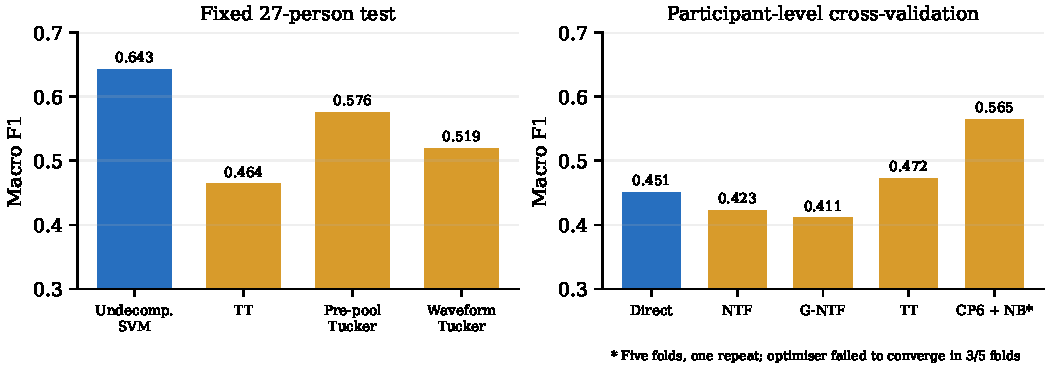
\includegraphics[width=0.92\textwidth]{figures/fig_tensor_results.pdf}
\caption{Tensor-decomposition ablations. Blue is the undecomposed spectral reference and gold denotes a tensor method. Fixed-split and cross-validated evidence are separated because their absolute values are not directly comparable. Low-rank compression did not improve the matched spectral baseline; CP6 + naive Bayes is the strongest adaptation but used only one five-fold run and had convergence failures.}
\label{fig:tensorresults}
\end{figure*}
\FloatBarrier

\paragraph{Outcome of the initial G-NTF hypothesis.} The planned advantage did not appear in the evaluation. G-NTF improved only marginally over plain NTF in balanced accuracy ($47.2\%$ versus $46.8\%$), had lower macro F1 ($41.1\%$ versus $42.3\%$), did not beat the shuffled-graph control, and remained below the undecomposed features. The optimisation was also unstable, with no converged start in 16 outer fits. We therefore reject the performance part of the original hypothesis for this cohort and protocol. The graph-constrained factors remain useful descriptively because they expose electrode, frequency and statistic patterns, but that interpretability must not be presented as evidence of better prediction.

\paragraph{Reading.} Under honest validation, neither CP nor TT beat the spectral baseline. CP gave interpretable, non-negative components but is non-convex, permutation-ambiguous and fragile to optimise; TT is stable but compressed away diagnostic variance at the ranks the development CV favoured. The tensor viewpoint remained valuable as a controlled ablation framework, but low-rank structure here removed class-relevant variance together with noise, and ranks selected on 26--147 people overfit. Section~\ref{sec:tensorinterp} opens the factors up to see what they encode.

\subsection{Interpretability analysis of the tensor factors}
\label{sec:tensorinterp}
Classification scores alone do not show \emph{what} a decomposition learned, so we examined the factors of each method: where on the scalp (electrode mode), at which frequencies (spectral mode), in which summary statistic, and how the participant-level scores differ between diagnoses. The analysis uses the saved final models (G-NTF on all 174 people; TT and Tucker fitted on the 147 development people) and is \emph{descriptive}: factors were fitted on people who also appear in the comparisons, class tests use Kruskal--Wallis with Benjamini--Hochberg (BH) correction, and none of it is held-out evidence. Electrode names follow the verified 10--20 order; mel-band centres in Hz are the 24 filter centres between 1 and 40 Hz; bands are delta (1--4), theta (4--8), alpha (8--13), beta (13--25) and gamma (25--40~Hz).

\paragraph{CP (graph-regularised NTF, rank 5).}
Each component is a product of an electrode map $\mathbf B_r$, a frequency curve $\mathbf F_r$ and a statistic profile $\mathbf S_r$, switched on in each person by an activation $A_{nr}$ (Fig.~\ref{fig:icp}, Table~\ref{tab:icp}). Reading the factors:
\begin{itemize}
\item \textbf{Component 1: temporal/frontal theta.} It peaks at 7.1~Hz and loads on T7, F7 and T8. Activation is highest in AD (median $16.4$ versus $12.2$ FTD and $12.7$ HC; AUC $0.71$ for AD versus HC and $0.72$ for AD versus FTD; FTD and HC are indistinguishable, AUC $0.50$). This is the classical AD theta increase.
\item \textbf{Component 2: occipital alpha.} It peaks at 10.2~Hz with O1, O2 and P8 dominant. Activation falls monotonically from HC ($14.4$) through FTD ($10.6$) to AD ($6.9$) (AUC for HC over AD $0.79$, $q=3.5{\times}10^{-7}$), i.e.\ posterior alpha loss, the other classical AD marker. It also correlates with MMSE across the 88 OpenNeuro participants ($\rho=0.53$, $q=3.3{\times}10^{-6}$), but this pooled correlation partly reflects the group difference and is exploratory.
\item \textbf{Components 3 and 4: low-frequency activity.} Their peaks lie at 2.5~Hz (F7/F8/Fp1 and Fp2/O1/O2) and they show no reliable group difference ($q=0.24$ and $0.61$). \textbf{Component 5} (a second alpha peak with a beta shoulder, T8/F7/T7) is borderline ($q=0.089$).
\item \textbf{Statistic profiles are almost flat.} Each of the mean, SD, median and IQR carries 23--29\% of the loading, so the components describe overall spectral level rather than a specific kind of variability across windows.
\end{itemize}
\emph{Stability.} We matched each of the 15 outer-fold factorisations to the full-cohort reference by Hungarian assignment. Components 3 and 2 recur in 14 and 13 folds (median product of cosine similarities $0.93$ and $0.87$) and component 4 in 11 ($0.86$), but components 1 and 5 recur only in 10 and 9 folds ($0.77$ and $0.82$). The best-objective final fit also stopped at its 250-iteration cap without a convergence flag, so the CP components should be read as one plausible solution, not a unique one (CP is permutation-ambiguous and non-convex).

\paragraph{Tensor Train (rank 4).}
The four TT features are contractions of the $19{\times}24{\times}4$ participant tensor with the shared core product; together they explain only $36.3\%$ of the centred variance (reconstruction error $63.7\%$). We characterised each feature by its \emph{energy share} over electrodes, bands and statistics (squared loadings), and mapped the linear-SVM weights back to the original electrode--frequency space as $\mathbf w=\mathbf V\,(\mathbf c/\boldsymbol\sigma)$, where $\mathbf V$ is the TT basis, $\mathbf c$ the SVM coefficients on standardised features and $\boldsymbol\sigma$ their scale; a positive weight pushes the prediction towards the first class of the pair (Fig.~\ref{fig:itt}, Table~\ref{tab:itt}).
\begin{itemize}
\item \textbf{Feature 3 (8.4\% variance)} is the main dementia axis: parietal (P3, P4, P7) delta--theta ($33\%$ of energy) versus beta ($37\%$), based on mean/median levels. Scores are highest in AD ($4.4$), intermediate in FTD ($-2.0$) and lowest in HC ($-8.3$), $p=1.9{\times}10^{-6}$.
\item \textbf{Feature 2 (10.8\%)} is a parietal variability feature (SD and IQR carry $71\%$ of its energy; theta and gamma dominated). It separates FTD (median $-6.4$) from AD ($+3.5$; $p=6.2{\times}10^{-4}$) and is the main contributor to the AD-versus-FTD decision.
\item \textbf{Feature 1 (13.2\%)} is a diffuse lateral-central high-frequency level (gamma $47\%$, beta $26\%$, alpha $17\%$) with weak class separation ($p=0.10$), and \textbf{feature 4 (3.9\%)} an occipital alpha--beta level that does not separate the classes ($p=0.26$).
\end{itemize}
Projected back to scalp--frequency space, the AD-versus-HC weights favour \emph{AD} for frontal theta ($+0.25$), frontal gamma ($+0.39$) and parietal theta ($+0.13$), and favour \emph{HC} for parietal beta ($-0.27$), occipital beta ($-0.16$) and posterior alpha ($-0.13$). Summed over electrodes the band totals are theta $+0.57$, gamma $+0.52$, alpha $-0.39$ and beta $-0.23$. FTD versus HC shares the alpha/beta loss (totals $-0.50$ each) with a smaller theta shift ($+0.23$); AD versus FTD is driven mainly by theta ($+0.51$, higher in AD). The frontal-gamma weight should be treated with caution, since muscle and acquisition noise also occupy this range.

\paragraph{Tucker/HOSVD (ranks $8{\times}16{\times}5$).}
The three factor matrices keep $77.8\%$ (electrode), $93.8\%$ (frequency) and $86.3\%$ (time) of the window variance (Fig.~\ref{fig:itk}). Electrode mode 1 ($41\%$ of electrode variance) is spatially uniform, i.e.\ overall level; mode 2 ($8\%$) is an anterior--posterior gradient (lateral frontal negative, occipital positive); mode 3 ($6\%$) contrasts central with frontal/occipital sites. Frequency mode 1 ($27\%$) is a high-frequency tilt, mode 2 ($20\%$) a low-versus-high contrast with a trough near 8~Hz, mode 3 ($12\%$) an alpha--beta pattern against slow activity (positive near 9~Hz and at 13--25~Hz, negative below 6~Hz), and mode 4 ($6\%$) an alpha peak plus gamma. To see which core coefficients carry diagnostic information we tested the participant-mean coefficient of each of the $8{\times}16$ electrode$\times$frequency mode pairs against diagnosis. Eight of the 128 pairs have BH-adjusted $q<0.05$, and one dominates: \textbf{uniform electrode mode 1 $\times$ frequency mode 3} ($p=1.2{\times}10^{-8}$, $q=1.6{\times}10^{-6}$), the global strength of the alpha--beta versus slow-activity pattern, which is the spectral slowing axis. The next-best pair has $q=0.020$.

\paragraph{Synthesis.}
All three decompositions tell the same story. The diagnostic content lies on a single spectral axis (slow theta activity versus alpha--beta activity, strongest over posterior regions and weakest for FTD), which matches the classical EEG signature of AD. In that sense the tensor factors are interpretable and neuroscientifically sensible. But they mainly re-express relative band power: spatial structure adds little beyond it (the CP statistic profiles are flat, the dominant Tucker electrode mode is spatially uniform and the TT electrode loadings are diffuse), FTD is separated from AD and HC only weakly, and the four TT features capture only about a third of the variance. This explains, mechanistically, why the decompositions matched but did not beat band-power-based spectral SVMs, and it shows that in this study the tensor viewpoint adds interpretability rather than accuracy.

\begin{figure*}[t]
\centering
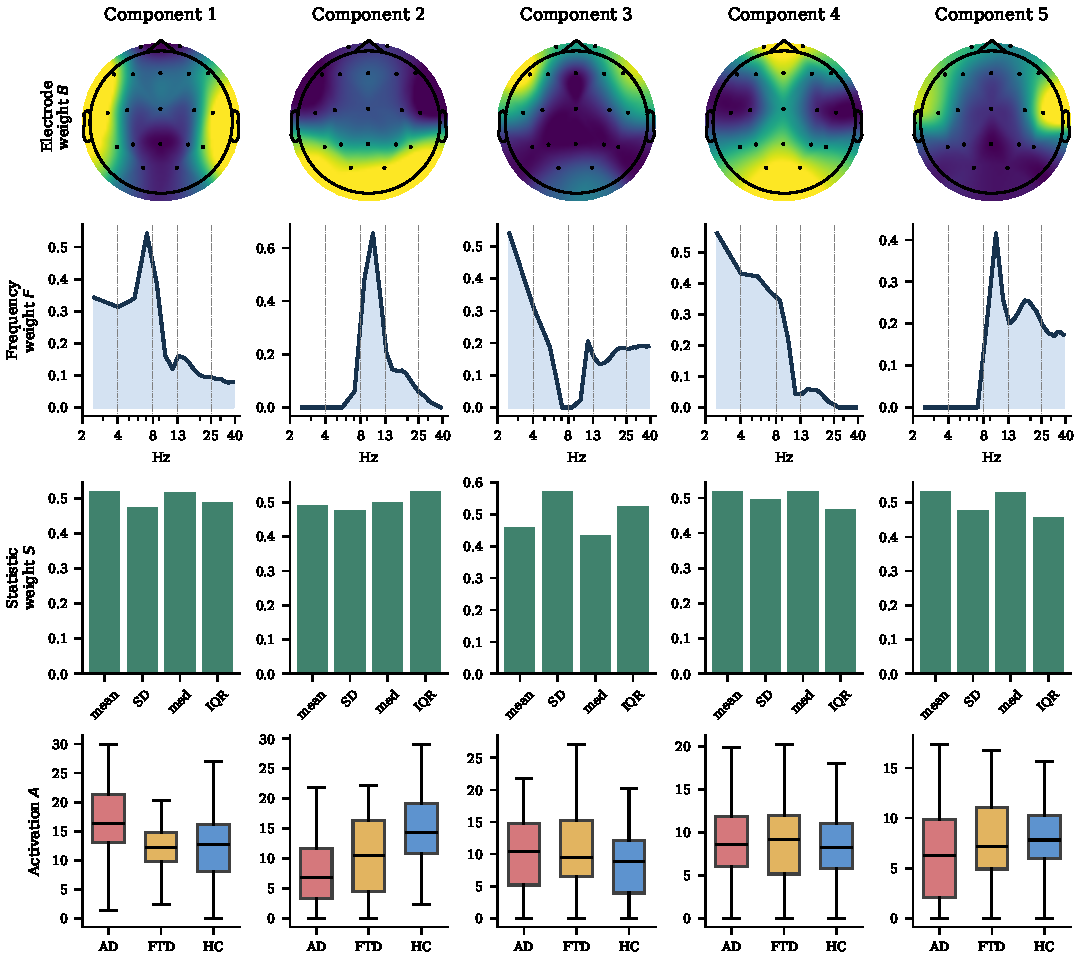
\includegraphics[width=0.88\textwidth]{figures/fig_interp_cp.pdf}
\caption{G-NTF (CP, rank 5) factors. Rows: electrode weights (scalp map), frequency weights (Hz; dotted lines mark the theta, alpha, beta and gamma boundaries), statistic weights, and participant activation by diagnosis (boxplots). Component 1 is a temporal/frontal theta component higher in AD; component 2 is an occipital alpha component that decreases from HC to FTD to AD.}
\label{fig:icp}
\end{figure*}

\begin{table*}[t]
\centering\scriptsize
\caption{CP components (graph-regularised NTF, rank 5, 174 people; descriptive). AUC is for AD scoring higher than HC; $q$ is the BH-corrected Kruskal--Wallis test over the three diagnoses; Folds is the number of the 15 outer-fold factorisations matched to the component; MMSE is Spearman $\rho$ across 88 OpenNeuro people ($q$ in brackets).}
\label{tab:icp}
\resizebox{\textwidth}{!}{%
\begin{tabular}{@{}clllcccc@{}}
\toprule
Comp.\ & Peak (Hz) & Top electrodes & Median activation AD / FTD / HC & AUC AD--HC & $q$ & Folds & MMSE $\rho$ ($q$)\\
\midrule
1 & 7.1 (theta) & T7, F7, T8 & 16.4 / 12.2 / 12.7 & 0.71 & $3.3{\times}10^{-5}$ & 10 & $-0.28$ (0.13)\\
2 & 10.2 (alpha) & O2, O1, P8 & 6.9 / 10.6 / 14.4 & 0.21 & $3.5{\times}10^{-7}$ & 13 & $+0.53$ ($3{\times}10^{-6}$)\\
3 & 2.5 (delta) & F7, F8, Fp1 & 10.4 / 9.4 / 8.9 & 0.57 & 0.24 & 14 & $-0.19$ (0.29)\\
4 & 2.5 (broad slow) & Fp2, O1, O2 & 8.6 / 9.2 / 8.3 & 0.55 & 0.61 & 11 & $-0.20$ (0.28)\\
5 & 10.2 (alpha+beta) & T8, F7, T7 & 6.2 / 7.2 / 7.8 & 0.39 & 0.089 & 9 & $+0.27$ (0.13)\\
\bottomrule
\end{tabular}}
\end{table*}

\begin{figure*}[t]
\centering
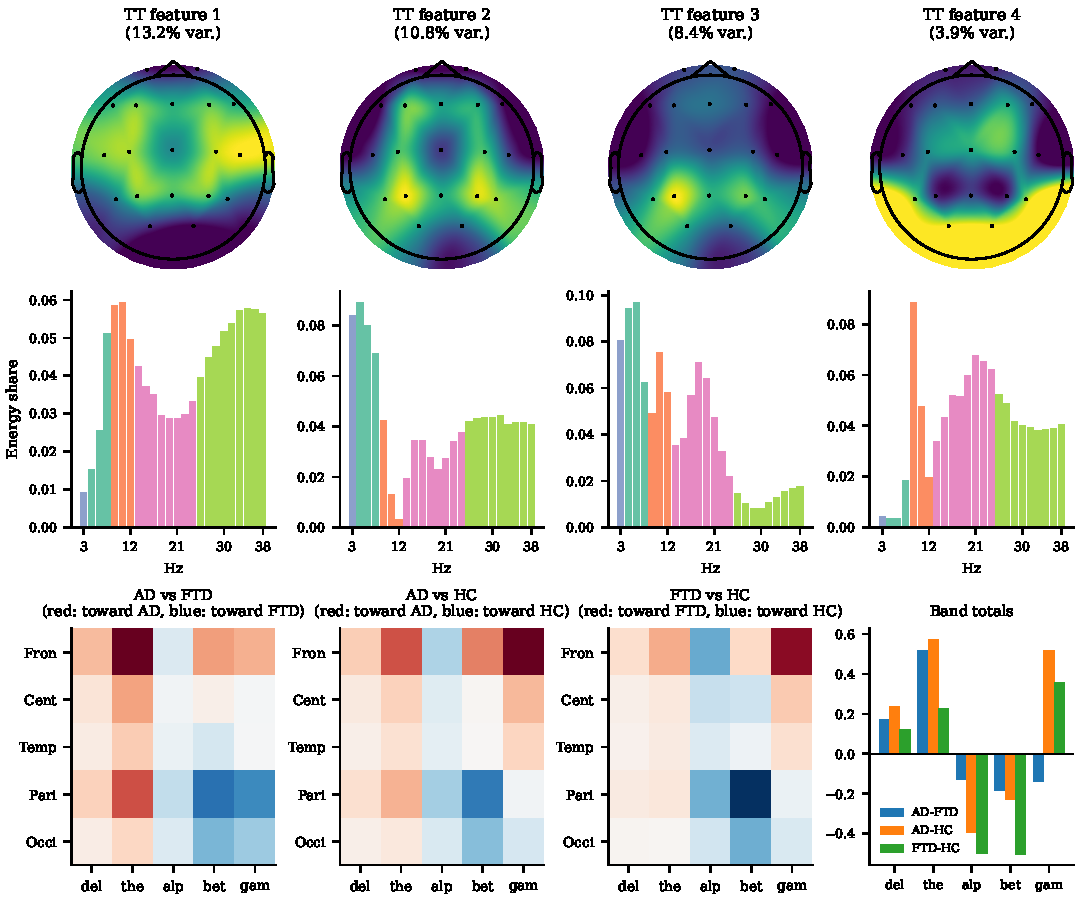
\includegraphics[width=0.88\textwidth]{figures/fig_interp_tt.pdf}
\caption{Tensor Train features (rank 4). Top: electrode energy share and, below, frequency energy share (bars coloured by band: delta, theta, alpha, beta, gamma). Bottom: linear-SVM weights mapped back to region$\times$band space for each class pair (red toward the first class, blue toward the second) and the band totals. AD is pushed by theta (and frontal gamma), HC by posterior alpha and beta.}
\label{fig:itt}
\end{figure*}

\begin{table*}[t]
\centering\small
\caption{Tensor Train features (final model on the 147 development people; descriptive). Energy shares are squared loadings; $p$ is an uncorrected Kruskal--Wallis test of the feature score across diagnoses.}
\label{tab:itt}
\begin{tabular}{@{}clllllc@{}}
\toprule
Feature & Variance & Top electrodes & Dominant bands (energy) & Statistics (energy) & Median score AD / FTD / HC & $p$\\
\midrule
1 & 13.2\% & T8, C4, C3 & gamma 47\%, beta 26\% & mean/median 74\% & $0.3$ / $2.5$ / $-1.4$ & 0.10\\
2 & 10.8\% & P3, P4, P8 & gamma 38\%, theta 24\% & SD/IQR 71\% & $3.5$ / $-6.4$ / $-2.0$ & $6.2{\times}10^{-4}$\\
3 & 8.4\% & P3, P4, P7 & beta 37\%, theta 25\% & mean/median 71\% & $4.4$ / $-2.0$ / $-8.3$ & $1.9{\times}10^{-6}$\\
4 & 3.9\% & O2, O1, P8 & beta 44\%, gamma 38\% & mean/median 90\% & $1.6$ / $0.1$ / $-1.0$ & 0.26\\
\bottomrule
\end{tabular}
\end{table*}

\begin{figure*}[t]
\centering
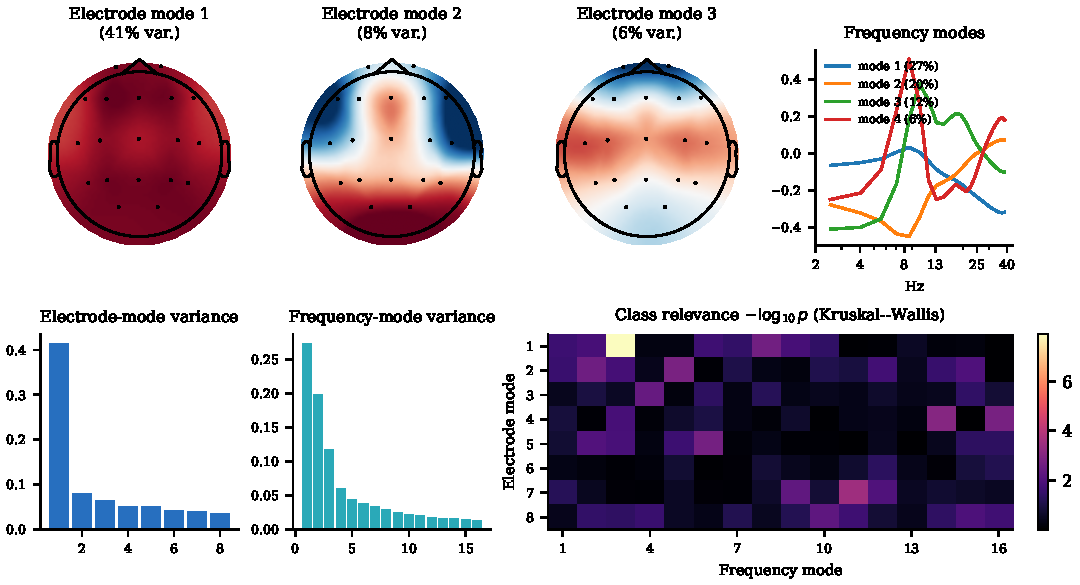
\includegraphics[width=0.88\textwidth]{figures/fig_interp_tucker.pdf}
\caption{Tucker/HOSVD factors (ranks $8{\times}16{\times}5$). Top: first three electrode modes (scalp maps) and the first four frequency modes with their variance share. Bottom: variance carried by each electrode and frequency mode, and class relevance of each electrode$\times$frequency mode pair (participant-mean coefficient; $-\log_{10}p$). Electrode mode 1 $\times$ frequency mode 3 is by far the most diagnostic pair.}
\label{fig:itk}
\end{figure*}

%% =====================================================================
\FloatBarrier
\raggedbottom
\section{Raw-Waveform 1D CNN}
\label{sec:cnn}
\subsection{Motivation and input}
The spectral pipeline fixes the representation (STFT, mel bank, summary statistics). We asked whether a network can learn temporal filters directly from the waveform. The input is the harmonised raw signal of Sec.~\ref{sec:prep}: $19\times1024$ windows (8~s at 128 Hz), $6{,}721$ windows from 174 participants, at most 40 per person, with the \emph{same} 121/26/27 participant split as Sec.~\ref{sec:threeclass}. No STFT, mel filterbank or MFCC is used. Each window is mean-removed and divided by a \emph{per-channel} standard deviation computed once on the training windows. During training we use gain jitter ($\pm10\%$), circular time shifts ($\pm0.25$~s), random single-channel dropout ($p{=}0.35$) and additive noise ($\sigma{=}0.015$).

\subsection{Architecture}
The compact network has \textbf{75,463 parameters}: (i) a depth-wise temporal convolution with four learned filters per electrode (kernel 65, $\approx$0.5~s), batch norm, GELU, a $1{\times}1$ mixing convolution to 64 channels and average pooling by 4; (ii) three depth-wise-separable blocks (64$\to$96, kernel 31; 96$\to$128, kernel 15; 128$\to$128, kernel 7; stride 2 each); (iii) concatenated global mean and max pooling and a 96-unit head (dropout 0.4) with three outputs. A second \textbf{multiscale attention-MIL} variant (148,524 parameters) uses parallel temporal kernels of 17/33/65/129 samples and learns attention weights \cite{ilse2018} over bags of eight windows from one participant, so the loss is applied at participant level.

\subsection{Training protocol}
AdamW (learning rate $10^{-3}$, weight decay $10^{-3}$, cosine decay), batch size 128, gradient clipping, mixed precision. Windows are sampled with weight inversely proportional to the participant's window count so each participant counts equally, and cross-entropy is weighted by class frequency. The checkpoint is chosen by \textbf{participant-level validation macro F1} (ties by balanced accuracy); a participant's prediction is the mean softmax over its windows. Three predetermined seeds are trained; the test set is used only after selection. A third protocol trains five CNNs for a fixed four epochs on participant-stratified folds of the 147 development people, giving one out-of-fold prediction for each of them and an averaged prediction for the 27 test people.

\subsection{Results}
\label{sec:cnnresults}
Table~\ref{tab:cnn} and Fig.~\ref{fig:cnnvar} summarise validation and test results.

\begin{table*}[!tbp]
\centering\small
\caption{Raw-waveform CNN results (participant level; fixed 27-person test split unless noted). Recall order is AD/FTD/HC. SVM reference is the log-mel SVM of Sec.~\ref{sec:threeclass}.}
\label{tab:cnn}
\begin{tabular}{@{}lccccc@{}}
\toprule
Model & Validation acc./F1 & Test acc. & Test BA & Test macro F1 & Test recall (\%)\\
\midrule
Window CNN, 3-seed mean & 57.7 / 52.2 & 59.3 & 58.5 & 57.5 & 45/50/80\\
Window CNN, validation-selected seed (ep.~4) & 69.2 / 61.4 & \textbf{70.4} & 70.1 & \textbf{69.6} & 64/67/80\\
Multiscale attention-MIL CNN (ep.~14) & 73.1 / 72.0 & 66.7 & 67.1 & 66.4 & 55/67/80\\
Fusion: 0.3 SVM + 0.6 CNN + 0.1 MIL & 80.8 / 77.6 & 70.4 & 70.1 & 69.3 & 64/67/80\\
Fusion, all models refit on 147 people & -- & 66.7 & 66.5 & 65.5 & 73/67/60\\
Five-fold CNN ensemble (test) & -- & 66.7 & 69.3 & 66.7 & 55/83/70\\
\quad same ensemble, out-of-fold on 147 dev.\ people & \multicolumn{5}{l}{acc.\ 66.0, BA 65.3, macro F1 64.3, recall 55/53/88}\\
\midrule
Log-mel SVM (reference) & -- & 66.7 & 64.2 & 64.3 & 73/50/70\\
MFCC SVM (reference) & -- & 59.3 & 58.2 & 58.5 & 55/50/70\\
\bottomrule
\end{tabular}
\end{table*}

\begin{figure}[!tbp]
\centering
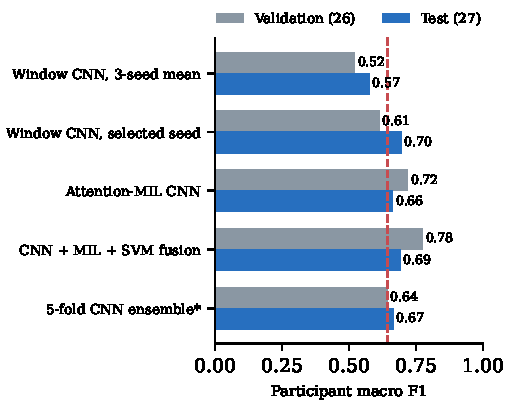
\includegraphics[width=\columnwidth]{figures/fig_cnn_variants.pdf}
\caption{Validation and test macro F1 of the raw-waveform CNN variants. *For the five-fold ensemble the grey bar is the out-of-fold development score (147 people). The dashed line is the log-mel SVM on the same test people.}
\label{fig:cnnvar}
\end{figure}

\paragraph{What looks interesting.} The raw-waveform CNN, with no hand-designed spectral stage, matches or exceeds the log-mel SVM: the validation-selected seed reaches $70.4\%$ test accuracy and macro F1 $0.696$, with FTD recall rising from $50\%$ (SVM) to $67\%$; fusing the CNN, MIL and SVM probabilities gives $80.8\%$ validation accuracy and $70.4\%$ on the test set; and the five-fold ensemble gives out-of-fold macro F1 $0.643$ on 147 people, consistent with $0.667$ on the test people. This out-of-fold figure is well above the $\approx0.50$ obtained by spectral SVMs under repeated CV. Other signals are less flattering: the best epoch is very early (4--14 epochs), so checkpoint choice matters, the three-seed average ($57.5$) is worse than the best single seed ($69.6$), and validation and test disagree in direction for the MIL model and the fusion (validation $72$--$78\%$ F1, test $66$--$69\%$), the usual winner's-curse pattern of selecting on 26 people.

\subsection{Per-site analysis}
\label{sec:cnnsite}
Because the cohorts differ in site, equipment and processing (Sec.~\ref{sec:brainlat}), we split the five-fold ensemble's predictions by site (out-of-fold for the 147 development people plus the averaged test predictions; 174 in all; Fig.~\ref{fig:site}).

\begin{figure*}[!tbp]
\centering
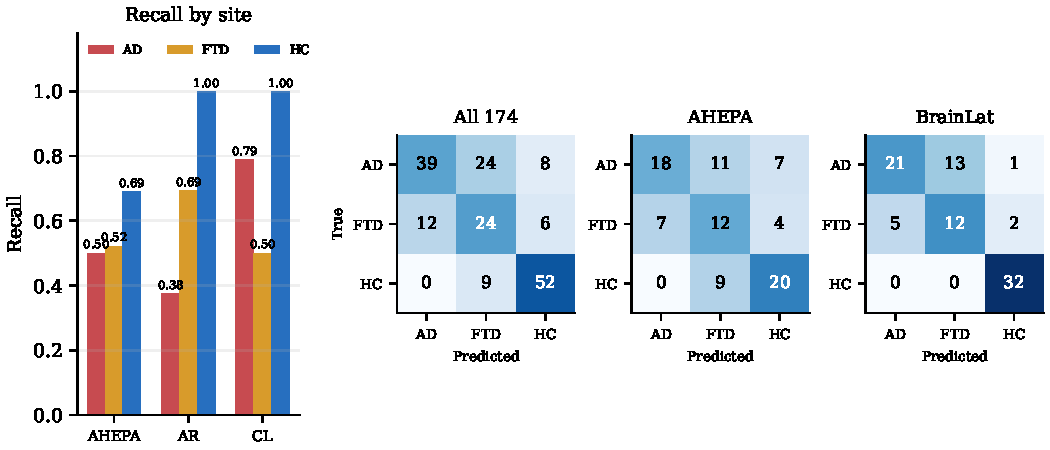
\includegraphics[width=0.94\textwidth]{figures/fig_site_audit.pdf}
\caption{Site audit of the five-fold raw CNN ensemble using out-of-fold development predictions plus averaged test predictions. Left: class recall at each site. Right: participant confusion matrices overall, at AHEPA and at the two BrainLat sites combined. All 32 BrainLat controls are classified as HC, whereas AHEPA control recall is $0.69$; this unusually clean separation is evidence of cohort dependence, not proof of clinical generalisation.}
\label{fig:site}
\end{figure*}

Three-class accuracy is $56.8\%$ in AHEPA but $75.6\%$ in BrainLat (AR $70.8\%$, CL $81.6\%$). Collapsed to HC-vs-dementia, the same predictions give $77.3\%$ accuracy in AHEPA but $96.5\%$ (balanced accuracy $97.2\%$) in BrainLat. BrainLat control recall is $32/32$. The CNN is thus far more accurate at the two BrainLat sites than at AHEPA, which is not the pattern shown by the log-mel SVM (Sec.~\ref{sec:binary}: macro F1 $0.76$ in AHEPA versus $0.63$--$0.64$ at AR and CL).

\subsection{OpenNeuro-only native-resolution control}
\label{sec:cnnopenneuro}
To test whether the CNN works without BrainLat, we trained on OpenNeuro only (88 people): native 19 channels, 500 Hz, no interpolation, resampling, extra filtering or re-referencing, 8~s windows ($19{\times}4000$), a CNN with a 251-sample first kernel (same blocks), stratified 60/14/14 train/validation/test participants. Results on the 14 test people were poor: the validation-selected model reached $42.9\%$ accuracy (BA $0.472$, macro F1 $0.427$; AD recall $0.17$), and the refit on all 74 development people reached $35.7\%$ accuracy (BA $0.389$). We then trained EEGPT only on the same OpenNeuro training split and selected a 50/50 probability blend on the validation participants. The blend improved test accuracy to $50.0\%$, BA to $0.556$ and macro F1 to $0.484$, but still recognised only one of six AD participants. EEGPT necessarily uses its pretrained 256 Hz input, while the CNN branch remains native 500 Hz. With 14 test people ($6/4/4$) the uncertainty is large (one person is $7.1$ points) and the split differs from the 27-person one, so this is \emph{not} proof of no signal; AHEPA-only OOF accuracy of $56.8\%$ in the larger experiment suggests some genuine signal. It does, however, remove the large performance advantage attributed to the waveform CNN.

\subsection{Interpretation}
The raw-waveform CNN delivers fixed-split numbers that match or exceed the spectral SVM, and its five-fold out-of-fold score is notably higher than anything spectral under repeated CV. But the per-site breakdown (controls $32/32$ in BrainLat; HC-vs-dementia $96.5\%$ vs.\ $77.3\%$) and the OpenNeuro-only control say that much of the gain comes from the BrainLat sites, as also happened with unnormalised EEGPT inputs (Sec.~\ref{sec:eegpt}). Blending the native CNN with EEGPT helps modestly on OpenNeuro ($42.9\%\to50.0\%$ accuracy) but does not solve the AD errors. We did not run leave-one-site-out or input-normalised versions of the CNN, so we cannot yet say how much of the gain would survive on an unseen site; those experiments are the necessary next step before the CNN can be preferred to the SVM.
\FloatBarrier
\flushbottom

%% =====================================================================
\FloatBarrier
\section{Discussion}
\label{sec:discussion}
\paragraph{Summary of the progression.} Table~\ref{tab:summary} collects the headline numbers. Estimates are only comparable within a protocol: moving from fixed split to repeated CV costs about 15 points of macro F1, and normalising the EEGPT inputs costs a further $\approx$10.

\begin{table*}[t]
\centering\small
\caption{Headline results across the project. ``Fixed'' = 27-person fixed split; ``CV'' = repeated participant-level cross-validation. Values are not directly comparable across rows.}
\label{tab:summary}
\begin{tabular}{@{}llllr@{}}
\toprule
Study & Task / cohort & Method & Protocol & Result\\
\midrule
Study I (V4) & 3-class, 88 & Tuned RBF SVM (spectral/TT) & 3$\times$5 CV, observed best & 59.7\% BA\\
Study I (V4) & 3-class, 88 & Whole-pipeline nested selection & 3$\times$5 nested CV & 54.5\% BA\\
Study I (V6) & HC vs.\ dem., 88 & 36 fixed pipelines & 3$\times$5 nested CV & 75.0\% acc., F1 0.718\\
Sec.~\ref{sec:binary} & HC vs.\ dem., 174 & Log-mel SVM, searched & 3$\times$5 nested CV & F1 0.699, BA 0.703\\
Sec.~\ref{sec:threeclass} & 3-class, 174 & Site-norm.\ log-mel SVM & Fixed & 66.7\% acc.\\
Sec.~\ref{sec:threeclass} & 3-class, 174 & Same SVM & 50 CV folds & F1 0.49\\
Sec.~\ref{sec:eegpt} & 3-class, 174 & SVM + EEGPT blend / frozen EEGPT & Fixed / CV & 70.4\% acc.\ / F1 0.60$\to$0.50\\
Sec.~\ref{sec:threeclass} & 3-class, 174 & Compact SVM/RF & 5$\times$5 CV & F1 0.51--0.52\\
Sec.~\ref{sec:tensor} & 3-class, 174 & TT, Tucker, CP/NTF/G-NTF & Fixed / CV & 52--59\% acc.\ / BA 0.47--0.51\\
Sec.~\ref{sec:tensor} & 3-class, 174 & CP6 + naive Bayes & 5-fold CV & 60.3\% acc., BA 0.565\\
Sec.~\ref{sec:cnn} & 3-class, 174 & Raw 1D CNN (selected) & Fixed & 70.4\% acc., F1 0.696\\
Sec.~\ref{sec:cnn} & 3-class, 174 & 5-fold raw CNN ensemble & OOF (147) / test (27) & F1 0.643 / 0.667\\
Sec.~\ref{sec:cnn} & 3-class, 88 & Native 500 Hz CNN & 14-person test & 42.9\% acc.\\
Sec.~\ref{sec:cnn} & 3-class, 88 & Native CNN + EEGPT blend & 14-person test & 50.0\% acc., F1 0.484\\
\bottomrule
\end{tabular}
\end{table*}

\paragraph{Why do tensors not help?} The data is tiny (42 FTD people), and low-rank bases fitted to it discard weak, class-relevant variance; selection among many ranks and classifiers on 26 validation people produces optimistic validation scores that do not carry over (waveform Tucker: validation F1 $81\%$, test $55\%$). The initial G-NTF hypothesis was not supported: its graph constraint did not outperform the shuffled-graph control, and CP factorisations added optimisation variance (no converged start in 16 G-NTF outer fits and 3 of 5 CP6 folds), while TT was stable but compressed away signal.

\paragraph{Site and protocol shift dominate.} Site-wise normalisation helped more than any model change, yet cohorts remain detectable after harmonisation, so a model can look good at one site for reasons that do not transfer. Spectral relative-power features still carry a consistent AD signal in all three sites (theta up, posterior alpha down), weaker in BrainLat, and are the part of the evidence we trust most.

\paragraph{Where the CNN stands.} The raw 1D CNN is attractive: compact, representation-free and quick to train (about 2 minutes for three seeds on a GPU). It is the only method whose out-of-fold macro F1 on 147 people ($0.643$) exceeds the spectral SVMs, but the per-site analysis shows this is driven by the BrainLat sites. The OpenNeuro-only EEGPT blend recovers only one extra correct participant and remains below 0.50 macro F1. Until the raw model is evaluated with leave-one-site-out or external data, its fixed-split number should be treated as a hypothesis-generating result, not the project benchmark.

%% =====================================================================
\section{Limitations}
\label{sec:limits}
\begin{itemize}
\item \textbf{No external validation.} All 174 participants were used in many iterations; nested CV cannot remove researcher-level adaptive exposure.
\item \textbf{Small test sets.} The 27-person split (6 FTD) has a 95\% interval of roughly 52--84\% around 70\%; one participant is 3.7 points.
\item \textbf{FTD scarcity.} Only 42 FTD participants exist; more windows do not add independent patients.
\item \textbf{Cohort confounds.} Different hospitals, amplifiers, references, upstream cleaning, EEGLAB versions and ages.
\item \textbf{Interpolation.} BrainLat channels are model-estimated, and inherited derivatives differ in cleaning between sources.
\item \textbf{Not clinical.} Labels are clinical diagnoses, and the models are research prototypes, not diagnostic tools.
\item \textbf{Not run.} Leave-one-site-out evaluation and repeated nested CV of the CNN, and an input-normalised variant of it.
\end{itemize}

%% =====================================================================
\section{Conclusion}
\label{sec:conclusion}
Starting from 88 OpenNeuro participants we reached about 60\% balanced accuracy with tuned SVMs; enlarging to 174 participants through BrainLat interpolation gave a log-mel SVM with $66.7\%$ fixed-split accuracy, an honest repeated-CV macro F1 near $0.50$ for three classes and $0.70$ for HC versus dementia. CP and Tensor-Train decompositions gave a rigorous but negative ablation; their factors are interpretable and recover the known AD signature (more theta, less posterior alpha), but they mostly re-express relative band power, which explains why they do not beat the spectral baseline. A raw-waveform 1D CNN gave the most striking validation and test numbers ($70.4\%$ test accuracy; out-of-fold macro F1 $0.643$), yet a per-site audit shows that its advantage sits at the BrainLat sites. On OpenNeuro alone the CNN reached $42.9\%$ accuracy and an EEGPT blend only $50.0\%$ on 14 test people. The defensible project contribution is therefore a transparent participant-level three-class baseline and a documented site-bias audit, not a state-of-the-art accuracy claim. The main lessons are methodological: use participant-level and nested protocols, report results site by site before trusting a gain, and re-test raw-waveform models with leave-one-site-out and genuinely external data.

%% =====================================================================
\section*{Author Contributions}
\phantomsection\label{sec:contrib}
\addcontentsline{toc}{section}{Author Contributions}
Table~\ref{tab:contrib} lists each author's roles and the parts of this report that document them; every section, figure and table number in the table is a link. Feature extraction is not listed as a separate role, because it is part of the spectral, tensor, baseline and deep-learning work of several authors. Vatipalli Abhiram led the project.

\begin{table*}[!t]
\centering\footnotesize
\caption{Author contributions. ``\S'' numbers link to the corresponding sections; ``Repro.''\ links to the Reproducibility statement.}
\label{tab:contrib}
\begin{tabular}{@{}p{0.2\textwidth}p{0.48\textwidth}p{0.26\textwidth}@{}}
\toprule
Author & Role & Where in this report\\
\midrule
\textbf{Vatipalli Abhiram} & Overall project supervision (project lead) & \sref{sec:intro}, \sref{sec:discussion}\\
24BDS087 & Evaluation protocol and leakage control (participant-level splits, nested and repeated CV) & \sref{sec:study1prep}, \sref{sec:logmel}, \sref{sec:repeatedcv}\\
 & Machine-learning and deep-learning model development and training on the local machine & \sref{sec:logmel}--\sref{sec:threeclass}, \sref{sec:cnn}\\
 & Spectral processing (STFT, log-mel representation) & \sref{sec:spectral}\\
 & Tensor construction (participant-level tensors and projection of held-out people), shared with Neeruganti Jeevan Sai & \sref{sec:tensorrecipe}, \sref{sec:cp}, \sref{sec:tt}\\
\midrule
\textbf{Neeruganti Jeevan Sai} & Tensor decomposition and interpretability: CP and graph-regularised NTF (shared role) & \sref{sec:cp}, \sref{sec:tensorresults}, \sref{sec:tensorinterp}\\
24BDS046 & Tensor construction, shared with Vatipalli Abhiram & \sref{sec:tensorrecipe}, \sref{sec:tt}\\
 & Site normalisation and harmonisation & \sref{sec:compat}, \sref{sec:logmel}\\
 & Study I tensor benchmark (88 participants, V1--V6) & \sref{sec:study1}\\
 & Ablation and electrode/frequency stability analysis & \sref{sec:interp}, \sref{sec:repeatedcv}, \sref{sec:eegpt}\\
 & Environment and compute setup & \reprolink\\
\midrule
\textbf{Palyam Maruthi} & Spatial interpolation (128$\to$19 electrodes) & \sref{sec:interp}\\
24BCS098 & Hyperparameter search & \sref{sec:study1}, \sref{sec:binary}\\
 & Literature review and paper replication & \sref{sec:litreview}, \sref{sec:litadapt}\\
 & Reproducibility and testing & \reprolink\\
 & Alternative baselines (Riemannian, MFCC, microstate, random forest) & \sref{sec:fixedsplit}, \sref{sec:repeatedcv}, \sref{sec:litadapt}, \sref{sec:cnnresults}\\
 & Presentation and demo handoff & (outside this report)\\
\midrule
\textbf{Kothapalli Tharun Chowdary} & Dataset collection (OpenNeuro and BrainLat) & \sref{sec:opn}, \sref{sec:brainlatdata}\\
24BDS032 & Initial dataset audit & \sref{sec:study1prep}, \sref{sec:compat}\\
 & Cleaning and preprocessing & \sref{sec:study1prep}, \sref{sec:prep}\\
 & Clinical metadata and label verification & \sref{sec:brainlatdata}, \sref{sec:compat}\\
 & Results and summarisation & \sref{sec:discussion}, Table~\ref{tab:summary}\\
 & Site-difference validation (per-site checks of model results and site-normalisation corrections) & \sref{sec:eegpt}, \sref{sec:cnnsite}, \sref{sec:cnnopenneuro}\\
\midrule
\textbf{Shaik Moiz} & Tensor decomposition and interpretability: Tensor Train and Tucker (shared role) & \sref{sec:tt}, \sref{sec:tucker}, \sref{sec:tensorinterp}\\
24BCS133 & Pretrained-model work (EEGPT) & \sref{sec:eegpt}\\
 & Report writing & \sref{sec:intro}--\sref{sec:conclusion}\\
 & Experiment record-keeping & \reprolink\\
 & Statistical analysis (repeated-CV spread, bootstrap intervals, FDR tests, per-site breakdowns) & \sref{sec:binary}, \sref{sec:repeatedcv}, \sref{sec:tensorinterp}\\
 & Figures and visualisation & Figs.~\ref{fig:pipeline}--\ref{fig:site}\\
\bottomrule
\end{tabular}
\end{table*}

%% =====================================================================
\section*{Reproducibility}
\phantomsection\label{sec:repro}
\addcontentsline{toc}{section}{Reproducibility}
The code, experiment configurations and result summaries behind this report are on the \code{research-validated-experiments} branch of \url{https://github.com/abhiram-v1/AIBSI}; its \code{README.md} maps every experiment in this report to its scripts and saved evidence and states which results were re-checked. Raw EEG is not redistributed: OpenNeuro \code{ds004504} and BrainLat must be obtained from their original sources. Code and outputs are in the project repository (\code{neural\_comparison/advanced\_clean\_spectral}, \code{binary\_logmel\_search}, \code{graph\_ntf\_svm}, \code{paper\_benchmark}, \code{dataset\_compatibility}, \code{tensor\_pipeline}). Raw-CNN scripts: \code{train\_raw\_1d\_cnn.py}, \code{evaluate\_raw\_1d\_cnn.py}, \code{train\_raw\_1d\_cnn\_mil.py}, \code{evaluate\_raw\_cnn\_fusion.py}, \code{evaluate\_raw\_1d\_cnn\_cv\_ensemble.py}, \code{train\_openneuro\_native\_1d\_cnn.py}, and \code{train\_openneuro\_native\_cnn\_eegpt\_blend.py}. The tensor interpretability figures and numbers come from \code{final\_report/tensor\_interpretability.py} (run with Python 3.10; it reads the saved G-NTF factors, the saved TT model and refits only the HOSVD covariance step). Other figures are regenerated by \code{final\_report/make\_figures.py} from saved outputs (per-site breakdown from saved participant probabilities and the waveform manifest).

\begin{thebibliography}{99}\footnotesize\setlength{\itemsep}{0pt}
\bibitem{jeong2004} J.~Jeong, ``EEG dynamics in patients with Alzheimer's disease,'' \emph{Clinical Neurophysiology}, vol.~115, no.~7, pp.~1490--1505, 2004.
\bibitem{dauwels2010} J.~Dauwels, F.~Vialatte, and A.~Cichocki, ``Diagnosis of Alzheimer's disease from EEG signals: Where are we standing?'' \emph{Current Alzheimer Research}, vol.~7, no.~6, pp.~487--505, 2010.
\bibitem{nishida2011} K.~Nishida \emph{et al.}, ``Differences in quantitative EEG between frontotemporal dementia and Alzheimer's disease as revealed by LORETA,'' \emph{Clinical Neurophysiology}, vol.~122, no.~9, pp.~1718--1725, 2011.
\bibitem{miltiadous2023} A.~Miltiadous \emph{et al.}, ``A dataset of scalp EEG recordings of Alzheimer's disease, frontotemporal dementia and healthy subjects from routine EEG,'' \emph{Data}, vol.~8, no.~6, p.~95, 2023. OpenNeuro \code{ds004504}.
\bibitem{miltiadous2021} A.~Miltiadous \emph{et al.}, ``Alzheimer's disease and frontotemporal dementia: A robust classification method of EEG signals and a comparison of validation methods,'' \emph{Diagnostics}, vol.~11, no.~8, p.~1437, 2021.
\bibitem{dice2023} A.~Miltiadous \emph{et al.}, ``DICE-Net: A novel convolution-transformer architecture for Alzheimer detection in EEG signals,'' \emph{IEEE Access}, 2023, doi:10.1109/ACCESS.2023.3294618.
\bibitem{rostamikia2024} M.~Rostamikia, Y.~Sarbaz, and S.~Makouei, ``EEG-based classification of Alzheimer's disease and frontotemporal dementia: a comprehensive analysis of discriminative features,'' \emph{Cognitive Neurodynamics}, vol.~18, no.~6, p.~3447, 2024, doi:10.1007/s11571-024-10152-7.
\bibitem{jiang2026} L.~Jiang, Y.~Chen, Y.~He, J.~Liang, X.~Zhao, X.~Guo \emph{et al.}, ``A two-stage EEG microstate fusion framework for dementia screening and Alzheimer's disease/frontotemporal dementia differentiation,'' \emph{Biosensors}, vol.~16, no.~5, art.~258, 2026, doi:10.3390/bios16050258.
\bibitem{li2024} W.~Li, Y.~Varatharajah, E.~Dicks, L.~Barnard, B.~H.~Brinkmann, D.~Crepeau \emph{et al.}, ``Data-driven retrieval of population-level EEG features and their role in neurodegenerative diseases,'' \emph{Brain Communications}, vol.~6, no.~4, fcae227, 2024, doi:10.1093/braincomms/fcae227.
\bibitem{prado2023} P.~Prado \emph{et al.}, ``The BrainLat project, a multimodal neuroimaging dataset of neurodegeneration from underrepresented backgrounds,'' \emph{Scientific Data}, vol.~10, 2023, doi:10.1038/s41597-023-02806-8.
\bibitem{kolda2009} T.~G.~Kolda and B.~W.~Bader, ``Tensor decompositions and applications,'' \emph{SIAM Review}, vol.~51, no.~3, pp.~455--500, 2009.
\bibitem{cong2015} F.~Cong, Q.-H.~Lin, L.-D.~Kuang, X.-F.~Gong, P.~Astikainen, and T.~Ristaniemi, ``Tensor decomposition of EEG signals: A brief review,'' \emph{J.\ Neurosci.\ Methods}, vol.~248, pp.~59--69, 2015.
\bibitem{cichocki2015} A.~Cichocki \emph{et al.}, ``Tensor decompositions for signal processing applications: From two-way to multiway component analysis,'' \emph{IEEE Signal Process.\ Mag.}, vol.~32, no.~2, pp.~145--163, 2015.
\bibitem{delathauwer2000} L.~De~Lathauwer, B.~De~Moor, and J.~Vandewalle, ``A multilinear singular value decomposition,'' \emph{SIAM J.\ Matrix Anal.\ Appl.}, vol.~21, no.~4, pp.~1253--1278, 2000.
\bibitem{oseledets2011} I.~V.~Oseledets, ``Tensor-train decomposition,'' \emph{SIAM J.\ Sci.\ Comput.}, vol.~33, no.~5, pp.~2295--2317, 2011.
\bibitem{cai2011} D.~Cai, X.~He, J.~Han, and T.~S.~Huang, ``Graph regularized nonnegative matrix factorization for data representation,'' \emph{IEEE Trans.\ Pattern Anal.\ Mach.\ Intell.}, vol.~33, no.~8, pp.~1548--1560, 2011.
\bibitem{barachant2012} A.~Barachant, S.~Bonnet, M.~Congedo, and C.~Jutten, ``Multiclass brain--computer interface classification by Riemannian geometry,'' \emph{IEEE Trans.\ Biomed.\ Eng.}, vol.~59, no.~4, pp.~920--928, 2012.
\bibitem{michel2018} C.~M.~Michel and T.~Koenig, ``EEG microstates as a tool for studying the temporal dynamics of whole-brain neuronal networks: A review,'' \emph{NeuroImage}, vol.~180, pp.~577--593, 2018.
\bibitem{schirrmeister2017} R.~T.~Schirrmeister \emph{et al.}, ``Deep learning with convolutional neural networks for EEG decoding and visualization,'' \emph{Human Brain Mapping}, vol.~38, no.~11, pp.~5391--5420, 2017.
\bibitem{lawhern2018} V.~J.~Lawhern \emph{et al.}, ``EEGNet: A compact convolutional neural network for EEG-based brain--computer interfaces,'' \emph{J.\ Neural Eng.}, vol.~15, no.~5, 056013, 2018.
\bibitem{roy2019} Y.~Roy \emph{et al.}, ``Deep learning-based electroencephalography analysis: A systematic review,'' \emph{J.\ Neural Eng.}, vol.~16, no.~5, 051001, 2019.
\bibitem{wang2024} G.~Wang \emph{et al.}, ``EEGPT: Pretrained transformer for universal and reliable representation of EEG signals,'' in \emph{Proc.\ NeurIPS}, 2024.
\bibitem{ilse2018} M.~Ilse, J.~Tomczak, and M.~Welling, ``Attention-based deep multiple instance learning,'' in \emph{Proc.\ ICML}, 2018.
\bibitem{varoquaux2018} G.~Varoquaux, ``Cross-validation failure: Small sample sizes lead to large error bars,'' \emph{NeuroImage}, vol.~180, pp.~68--77, 2018.
\bibitem{cawley2010} G.~C.~Cawley and N.~L.~C.~Talbot, ``On over-fitting in model selection and subsequent selection bias in performance evaluation,'' \emph{J.\ Mach.\ Learn.\ Res.}, vol.~11, pp.~2079--2107, 2010.
\bibitem{johnson2007} W.~E.~Johnson, C.~Li, and A.~Rabinovic, ``Adjusting batch effects in microarray expression data using empirical Bayes methods,'' \emph{Biostatistics}, vol.~8, no.~1, pp.~118--127, 2007.
\bibitem{sun2016} B.~Sun, J.~Feng, and K.~Saenko, ``Return of frustratingly easy domain adaptation,'' in \emph{Proc.\ AAAI}, 2016, pp.~2058--2065.
\bibitem{pion2019} L.~Pion-Tonachini, K.~Kreutz-Delgado, and S.~Makeig, ``ICLabel: An automated EEG independent component classifier,'' \emph{NeuroImage}, vol.~198, pp.~181--197, 2019.
\bibitem{gramfort2013} A.~Gramfort \emph{et al.}, ``MEG and EEG data analysis with MNE-Python,'' \emph{Front.\ Neurosci.}, vol.~7, p.~267, 2013.
\bibitem{perrin1989} F.~Perrin, J.~Pernier, O.~Bertrand, and J.~F.~Echallier, ``Spherical splines for scalp potential and current density mapping,'' \emph{Electroencephalogr.\ Clin.\ Neurophysiol.}, vol.~72, pp.~184--187, 1989.
\bibitem{cortes1995} C.~Cortes and V.~Vapnik, ``Support-vector networks,'' \emph{Machine Learning}, vol.~20, pp.~273--297, 1995.
\end{thebibliography}

%% =====================================================================
\section*{Reference Usage Summary}
\phantomsection\label{sec:refusage}
\addcontentsline{toc}{section}{Reference Usage Summary}
Table~\ref{tab:refusage} summarises what this project took from each reference and where that material appears. Reference and section numbers are links. ``Used'' means the work's data, method or software was applied in our experiments. ``Adapted'' means we re-implemented a published method under our own protocol. ``Background'' means it informed the motivation or interpretation only.

\begin{table*}[!t]
\centering\footnotesize
\caption{What we took from each reference and where it is used in this report.}
\label{tab:refusage}
\begin{tabular}{@{}p{0.05\textwidth}p{0.08\textwidth}p{0.59\textwidth}p{0.18\textwidth}@{}}
\toprule
Ref. & Type & What we took from it & Where used\\
\midrule
\multicolumn{4}{@{}l}{\emph{Datasets and upstream processing}}\\
\cite{miltiadous2023} & Used & OpenNeuro \code{ds004504}: 88 AHEPA recordings (36 AD, 23 FTD, 29 CN) and the authors' cleaned EEGLAB derivatives & \sref{sec:litreview}, \sref{sec:opn}\\
\cite{prado2023} & Used & BrainLat AD, bvFTD and control EEG from Argentina and Chile (128-channel BioSemi, 512 Hz) & \sref{sec:litreview}, \sref{sec:brainlatdata}\\
\cite{pion2019} & Used & ICLabel artefact-component rejection, applied upstream by the dataset authors; we did not repeat it & \sref{sec:opn}\\
\cite{gramfort2013} & Used & MNE-Python for loading recordings, montages and \code{interpolate\_to} & \sref{sec:interp}\\
\cite{perrin1989} & Used & Spherical-spline interpolation for mapping 128 BrainLat channels to the 19-electrode montage and for bad-channel repair & \sref{sec:interp}, \sref{sec:prep}\\
\midrule
\multicolumn{4}{@{}l}{\emph{Clinical EEG background}}\\
\cite{jeong2004} & Background & AD slows the resting rhythm: more delta/theta, less posterior alpha/beta & \sref{sec:litreview}, \sref{sec:tensorinterp}\\
\cite{dauwels2010} & Background & Review of EEG-based AD diagnosis; spectral slowing and reduced coherence as markers & \sref{sec:litreview}, \sref{sec:tensorinterp}\\
\cite{nishida2011} & Background & FTD shows smaller, more frontal EEG changes than AD, which explains why FTD is the hardest class & \sref{sec:litreview}, \sref{sec:repeatedcv}\\
\midrule
\multicolumn{4}{@{}l}{\emph{Published classifiers compared or adapted}}\\
\cite{miltiadous2021} & Background & Comparison of validation schemes on the AHEPA data; supports participant-level splits throughout & \sref{sec:litreview}, \sref{sec:study1prep}\\
\cite{dice2023} & Adapted & DICE-Net (band power + coherence, convolution--transformer), re-headed for three classes & \sref{sec:litreview}, \sref{sec:litadapt}\\
\cite{rostamikia2024} & Adapted & Hierarchical handcrafted-feature SVM (dementia vs.\ HC, then AD vs.\ FTD) & \sref{sec:litreview}, \sref{sec:litadapt}\\
\cite{jiang2026} & Adapted & Two-stage EEG-microstate fusion cascade; the closest three-class endpoint to ours & \sref{sec:litreview}, \sref{sec:litadapt}\\
\cite{li2024} & Adapted & Non-negative CP of channel$\times$frequency spectra (rank 6) + naive Bayes; inspired the CP6 experiment & \sref{sec:litadapt}, \sref{sec:cp}\\
\midrule
\multicolumn{4}{@{}l}{\emph{Tensor methods}}\\
\cite{kolda2009} & Used & CP and Tucker definitions, notation and $n$-mode products & \sref{sec:tensorrecipe}, \sref{sec:cp}\\
\cite{cong2015} & Background & Review of tensor decomposition for EEG; supports the multi-way EEG view & \sref{sec:litreview}\\
\cite{cichocki2015} & Background & Tensor decompositions for signal processing; CP/Tucker interpretation & \sref{sec:litreview}\\
\cite{delathauwer2000} & Used & HOSVD for the pre-pooling Tucker factors & \sref{sec:tucker}, \sref{sec:tensorinterp}\\
\cite{oseledets2011} & Used & TT-SVD algorithm for the Tensor Train pipeline & \sref{sec:tt}, \sref{sec:tensorinterp}\\
\cite{cai2011} & Used & Graph-Laplacian regularisation, transferred from NMF to our graph-regularised non-negative CP (G-NTF) & \sref{sec:litreview}, \sref{sec:cp}\\
\midrule
\multicolumn{4}{@{}l}{\emph{Classifiers, baselines and deep learning}}\\
\cite{cortes1995} & Used & Support-vector machine, the main classifier & \sref{sec:logmel}--\sref{sec:threeclass}\\
\cite{barachant2012} & Used & Riemannian (covariance-based) classification for the filter-bank Riemannian SVM baseline & \sref{sec:fixedsplit}\\
\cite{michel2018} & Background & Microstate analysis, underlying the microstate baseline and the Jiang adaptation & \sref{sec:litreview}, \sref{sec:litadapt}\\
\cite{schirrmeister2017} & Background & CNNs learning temporal/spatial filters from raw EEG; motivated the raw-waveform CNN & \sref{sec:litreview}, \sref{sec:cnn}\\
\cite{lawhern2018} & Background & EEGNet's compact depth-wise/separable convolutions, a design similar to our raw CNN & \sref{sec:litreview}, \sref{sec:cnn}\\
\cite{roy2019} & Background & Review of deep learning for EEG; cautions on small cohorts and validation & \sref{sec:litreview}\\
\cite{wang2024} & Used & EEGPT pretrained checkpoint, frozen embeddings and partial fine-tuning & \sref{sec:eegpt}, \sref{sec:cnnopenneuro}\\
\cite{ilse2018} & Used & Attention-based multiple-instance pooling for the multiscale attention-MIL CNN & \sref{sec:cnn}\\
\midrule
\multicolumn{4}{@{}l}{\emph{Evaluation and site harmonisation}}\\
\cite{varoquaux2018} & Background & Small-sample CV has wide error bars; why we report repeated CV and not one split & \sref{sec:litreview}, \sref{sec:repeatedcv}\\
\cite{cawley2010} & Background & Selection bias without nested CV; why all selection is nested & \sref{sec:litreview}, \sref{sec:logmel}\\
\cite{johnson2007} & Background & ComBat batch-effect correction, as context for site harmonisation (not run in the reported experiments) & \sref{sec:litreview}\\
\cite{sun2016} & Used & CORAL alignment, tested in the cross-cohort compatibility audit & \sref{sec:litreview}, \sref{sec:compat}\\
\bottomrule
\end{tabular}
\end{table*}

\end{document}
